In Figure~\ref{fig:ck} we present the Count-Keeper (CK) data structure.  At a high level, CK uses information from both CMS and HK (with $d=1$) to create frequency estimates that are more accurate than either CMS or HK (alone) when the stream is ``honest", and that are more robust in the presence of adversarial streams.  After describing the structure, we will provide analytical support for its design, i.e., why it is more accurate and robust.  To summarize this very briefly and informally: CK is more accurate because its HK component can decrease the effect of ``collision noise" that drives up the values held at the relevant $M[i][p_i]$ in the CMS component; and it is more robust because a 1-cover no longer suffices to create estimation errors (minimally, a 2-cover is needed) and, unlike either CMS or HK alone, CK can detect when the state of $M,A$ is ``abnormal" and prone to producing spurious estimates.

\subsection{Structure}
At initialization, the CK initializes a standard CMS (initialized in the structure as~$M$) and a HK with the decay parameter~$d=1$ (initialized in the structure as~$A$) in their usual way. We set the substructures to be of the same number of rows and buckets and let the elements hash to the same counters' positions in each substructure using the same row hash functions. 

%The update procedure for the CK is a combination of that of the CMS and HK.
%, except for the latter case, we drop the notion of probabilistic decay (i.e., setting $d=1$).
% and just always decrement the counter on a fingerprint mismatch.
To insert a stream element~$x$ arrives, we run the CMS and HK update procedures $M\gets\Up^{\CMS}_{K}(M,\up_x)$ and $A\gets\Up^{\HK}_{K}(M,\up_x)$, respectively.  We note that the same positions $(p_1,\ldots,p_k) \gets R(K,x)$ are visited in both procedures; thus the same elements are observed by $M[i][p_i]$ and $A[i][p_i]$.  By ``observed", we mean that both $M[i][p_i]$ and $A[i][p_i]$ maintain summary information about the same substream, namely the substream of elements~$z$ such that $p_i\,{=}\,R(K,z)[i]$.


\begin{figure}[h]
	\Wider[3em]{
		\centering
		\begin{pcvstack}[boxed,center,space=0.5em]
			\begin{pchstack}
				\begin{pcvstack}[space=0.45em]
					\procedure[linenumbering, headlinecmd={\vspace{.1em}\hrule\vspace{.2em}}]{$\Rep_K(\setS)$}{%
						M \gets \zeros(k,m)\\
%						\pcgraycomment{$k\times m$ (fp,cnt) 2-d array}\\
						\pcfor i \in [k] \\
						\t A[i] \gets [(\star,0)]\times m\\
						\repr \gets \langle M,A\rangle\\
						\pcfor x \in \setS \\
						\t \repr \, {\getsr} \Up_K(\repr,{\up_{x}})\\
						\pcreturn \repr
					}
					\procedure[linenumbering, headlinecmd={\vspace{.1em}\hrule\vspace{.2em}}]{$\Up_K(\repr,\up_x)$}{%
						\langle M,A\rangle \gets \repr\\
						M  \getsr \Up^\CMS_{K}(M ,\up_x)\\
						A \getsr \Up^\HK_{K}(A ,\up_x)\\
						\pcreturn \repr {\gets}  \langle M,A\rangle
					}
				\end{pcvstack}
				\begin{pcvstack}[space=0.45em]
					\procedure[linenumbering, headlinecmd={\vspace{.1em}\hrule\vspace{.2em}}]{$\Qry_K(\repr,\qry_x)$}{%
						\langle M, A \rangle \gets \repr\\
						(p_1,\ldots,p_k) \gets R(K,x), \, \mathrm{fp}_{x} \gets T(K,x)\\
						\Theta_1,\Theta_2 \gets \infty\\
						\pcgraycomment{CMS only overestimates}\\
						\cnt_{\text{UB},x}\gets \Qry^\CMS_{K}(M,\qry_x) \\ %\label{line:ck:cms}\\
						\pcgraycomment{HK only underestimates}\\
						\cnt_{\text{LB},x} \gets \Qry^\HK_{K}(A,\qry_x) \\ %\label{line:ck:finalunderest}\\
						\pcgraycomment{return upperbound if equal to lowerbound}\\
						\pcif \cnt_{\text{UB},x} =  \cnt_{\text{LB},x}\\ %\label{line:UB=LB:start}\\
						\t \pcreturn \cnt_{\text{UB},x} \\ %\label{line:UB=LB:finish}\\
						\pcfor i \in [k]  \\ %\label{line:ck:startoverestdjust}\\
						\t \pcgraycomment{if never observed}\\
						\t \pcif A[i][p_i].\mathrm{fp} = \star\\
						\t \t \cnt_{\text{UB},x} \gets  0\\
						\t \t \pcreturn 0 \\ %\label{line:ck:est0}\\
						\t \pcgraycomment{upper bound adjustment}\\
						\t \pcgraycomment{x does not own counter}\\
						\t \pcelse \pcif A[i][p_i].\mathrm{fp} \not= \fp_x\\
						\t \t \Theta \gets \frac{M[i][p_i] {-} A[i][p_i].\cnt {+}1}{2}\\
						\t \t \Theta_1 {\gets} {\min}\left\{ \Theta_1, \Theta \right\}\\
%						\t \t \Theta_1 {\gets} 
%						{\min}\left\{ 
%						\Theta_1, \frac{M[i][p_i] {-} A[i][p_i].\cnt {+}1}{2}
%						\right\}\\
						\t \pcgraycomment{x owns counter}\\
						\t \pcelse \pcif A[i][p_i].\mathrm{fp} = \fp_x\\
						\t \t \Theta \gets \frac{M[i][p_i] {+} A[i][p_i].\cnt}{2}\\
						\t \t \Theta_2 {\gets} 
						{\min}\left\{ 
						\Theta_2, \Theta\right\}\\
%                         \t \t \Theta_2 {\gets} 
%						{\min}\left\{ 
%						\Theta_2, \frac{M[i][p_i] {+} A[i][p_i].\cnt}{2}
%						\right\}\\
						\cnt_{\text{UB},x} {\gets} \floor(\min\left\{ \Theta_1, \Theta_2 \right\}) \\%\label{line:ck:finaloverest}\\
						\pcreturn \cnt_{\text{UB},x}
					}
				\end{pcvstack}
			\end{pchstack}	
		\end{pcvstack}
	}
	\caption[The Count-Keeper Structure.]{Keyed structure $\CK[R,T,m,k]$ supporting point-queries for any potential stream element~$x$ ($\qry_x$).
		$\Qry^\CMS_{K}, \Up^\CMS_{K}$, resp. $\Qry^\HK_{K},  \Up^\HK_{K}$, denote query and update algorithms of keyed structure $\CMS[R,T,m,k]$ (Figure \ref{fig:cms}), resp. $\HK[R,T,m,k,1]$ (Figure \ref{fig:hk}, but note $d=1$). 
		The parameters are a function $R: \keys\by\bits^* \to [m]^k$, a function $T: \keys\by\bits^* \to \bits^n$ for some desired fingerprint length~$n$, and integers $m,k \geq 0$. A concrete scheme is given by a particular choice of parameters.}
	\label{fig:ck}
\end{figure}
%\eject



When queried for the frequency estimate of an element $x\in \set{U}$, CK first computes the CMS and HK estimates, which we will write as CMS($x$) and HK($x$) for brevity. If CMS($x$)=HK($x$), then we return their shared response.  We will see precisely why this is the correct thing to do, but loosely, it is because (under the NFC assumption) $\HK(x) \leq n_x \leq \CMS(x)$.  If $\CMS(x) \neq \HK(x)$ then CK proceeds row-by-row, using the information held at $A[i][p_i]$ to refine the summary information held at $M[i][p_i]$.  
If any of the $A[i][p_i].\fp$ are uninitialized, then we are certain that~$n_x=0$; had \emph{any} stream element been mapped to this position, the fingerprint would no longer be uninitialized.
%\footnote{Equivalently, we could conclusively return zero if any of the $M[i][p_i]=0$.}
In this case, CK($x$) returns 0.

%To explain this, recall our previously established notation $V^i_{x}\,{=}\,\{y \neq x \in \streamvar{S} \;|\; R(y)[i]=p_i=R(x)[i]\}$, i.e., the
%set of elements that ``collide" with a target element~$x$ in the CK structure. In particular, note that 
%if $y \in V^i_x$ then~$y$ covers the $i$-th row counter associated to~$x$, in both the CMS and HK portions of CK.

Now assume that none of the $A[i][p_i]$ have uninitialized fingerprints, and $\CMS(x) \neq \HK(x)$. To explain our row-by-row refinements, let us define two sets  
$I_x\,{=}\,\{i \in [k] \;|\; A[i][p_i].\fp\,{=}\,\fp_x \}$ and $\hat{I}_x\,{=}\,\{i \in [k] \;|\; A[i][p_i].\fp \neq \fp_x \}$, 
i.e., the subset of rows in~$M$ (and~$A$) that are ``owned" and not ``owned" (resp.) by~$x$.  
Observe that we can write the CMS estimate for~$x$ as
\[
\mathrm{CMS}(x)
%=\min_{i \in [k]}\{M[i][p_i ]\}
=\min \left\{    
\min_{i \in I_x}\left\{M[i][p_i]  \right\},
\min_{i \in \hat{I}_x}\left\{M[i][p_i]  \right\}
\right\}
\]
so for each row $i\in[k]$, we have two cases to consider.  For each case, CK maintains an internal estimator: when $i \in \hat{I}_x$ the estimator is~$\Theta^i_1$, and when $i \in I_x$ the estimator is $\Theta^i_2$.  We will talk about each of these, next. The upshot of this discussion is that CK defines $\Theta_1\,{=}\,\min_{i \in \hat{I}_x}\{\Theta^i_1\}$, $\Theta_2\,{=}\,\min_{i \in I_x}\{\Theta^i_2\}$, and its return value $\lfloor\min\{\Theta_1,\Theta_2\}\rfloor$ is always at least as good as $\CMS(x)$.  
% Later we will argue that the CK estimate can be significantly more precise than the CMS estimate.\tsnote{What about the HK estimate?!}  
 

\subsection{Correcting CMS and Correctness of CK}
In what follows, we will assume the NFC condition. For sufficiently large fingerprints (e.g., $\tau$-bit fingerprints where $2^\tau$ is much larger than the number of distinct elements in the stream) this is reasonable.  Under this assumption, CK may only overestimate the value of~$n_x$.

%\mia{Tom: Make sure that we point out we cover all the cases with the thetas. Most of it is already in the below; possibly add one 'killer' sentence.}
\paragraph{Correcting ${M[i][p_i]}$ when ${x}$ does not ``own" ${A[i][p_i]}$}
By its design as a count-all structure, the value of $M[i][p_i]=n_x + \sum_{y \in V^i_x}n_y$.  When $i \in \hat{I}_x$, we claim that $n_x \leq \sum_{y \in V^i_x}n_y$.  To see this, observe that if $n_x > \sum_{y \in V^i_x}n_y$ then~$x$ \emph{would} own $A[i][p_i]$: we can pair up appearances of~$x$ with appearances of elements in $y \in V^i_x$, and because no element of $V^i_x$ has the same fingerprint as~$x$, each pair $(x,y)$ effectively contributes 0 to the value of $A[i][p_i].\cnt$. So if $n_x > \sum_{y \in V^i_x}n_y$, the fingerprint held at $A[i][p_i]$ would be $\fp_x$.  Note that if $n_x\,{=}\,\sum_{y \in V^i_x}n_y$ and $i \in \hat{I}_x$, then $A[i][p_i].\cnt=1$ and some $y \neq x$ was the last insertion.  Thus, $A[i][p_i]-1$ is a lowerbound on the difference $\sum_{y \in V^i_x}n_y - n_x$, i.e., the number of occurrences of $y \in V^i_x$ that are not canceled out by an occurrence of~$x$.  Thus, $n_x + A[i][p_i]-1 \leq \sum_{y \in V^i_x}n_y$, which implies that $M[i][p_i]=n_x + \sum_{y \in V^i_x}n_y \leq 2n_x + A[i][p_i]-1$.
%

\begin{restatable}{lemma}{lmaThetaOne}\label{lma:fx:MA:Theta1}
	Let~$\streamvar{S}$ satisfy the NFC condition, and let $x \in \set{U}$.  Then for any $i \in \hat{I}_x$ we have
	$n_x \leq \frac{M[i][p_i] - A[i][p_i].\cnt +1}{2}\,{=}\,\Theta^i_1$.
	\hfill$\blacklozenge$
\end{restatable}

\begin{proof}[Proof of Lemma~\ref{lma:fx:MA:Theta1}]
    We can think of the counter $A[i][p_i].\cnt$ as counting the depth of a stack of fingerprint-labeled plates.  The rules of the stack are as follows.  Upon insertion of~$x$ into the CK structure: 
    \begin{enumerate}
        \item[1.] if $A[i][p_i].\cnt=0$ then the stack is empty; then push an $\fp_x$-labeled plate and set $A[i][p_i].\cnt \gets 1, A[i][p_i].\fp \gets\fp_x$.
        \item[2(a).] if $A[i][p_i].\cnt=c>0$ and $A[i][p_i].\fp =\fp_x$, then push an $\fp_x$-labeled plate on to the stack and increment $A[i][p_i].\cnt \gets c+1$.
        \item[2(b).]if $A[i][p_i].\cnt=c > 0$ and $A[i][p_i].\fp \neq \fp_x$, then pop the top ($\fp$-labeled) plate and decrement $A[i][p_i].\cnt \gets c-1$.  If this causes $A[i][p_i].\cnt=0$, then push an $\fp_x$-labeled plate and set $A[i][p_i].\cnt\gets 1, A[i][p_i].\fp \gets \fp_x$.
    \end{enumerate}
    These stack rules are precisely the CK rules for handling insertions.  Now, upon the first insertion to CK, by rule 1 it is clear that all plates on the stack (there is only one of them) have label $A[i][p_i].\fp$, and $A[i][p_i].\cnt$ is the number (1) of plates on the stack.  Inductively, assume that $A[i][p_i].\cnt=c>0$ and all~$c$ of the 
    plates on the stack have the same label $A[i][p_i].\fp$.  Say that the next insertion is~$z$ and $A[i][p_i].\fp=\fp_z$.  By rule 2(a), we push an $\fp_z$-plate on to the stack and increment $A[i][p_i].\cnt \gets c+1$.  In this case, by assumption, it remains the case that all 
    plates have the same label equal to $A[i][p_i].\fp$, and there are $c+1$ of them. Alternatively, if $ A[i][p_i].\fp \neq \fp_z$ then by rule 2(b) we pop the top plate and decrement $A[i][p_i].\cnt \gets c -1$.  At this point, either the stack is empty and $A[i][p_i].\cnt=0$, 
    so by 2(b) we push an $\fp_z$-plate and set $A[i][p_i].\cnt \gets 1$ and $A[i][p_i].\fp \gets \fp_z$; or the stack is not empty, and we take no further action.  In the first case, the stack contains a single plate labeled with $A[i][p_i].\fp$ and the 
    counter is 1; in the second, by assumption all plates on the stack are still labeled with  $A[i][p_i].\fp$, and $A[i][p_i].\cnt$ still gives the number of plates on the stack.
    
    Having shown the invariant of the stack, we make the following observation.  
    Let $\tilde{n} =  \sum_{y\in V_x^i} n_y$. Then $M[i][p_i] = n_x + \tilde{n}$. By the statement of the lemma $i \in \hat{I}_x$, implying that $A[i][p_i].\fp \neq \fp_x$.  
    We claim that $A[i][p_i].\cnt=c>0$ implies $\tilde{n}-n_x \geq A[i][p_i].\cnt-1$. To see this, note that $A[i][p_i].\cnt=c>0$ means that there are~$c$ plates labeled with~$A[i][p_i].\fp \neq \fp_x$ on the stack associated to $c$ insertions of elements in $V_x^i$ with fingerprint $A[i][p_i].\fp$. If there ever were any $\fp_x$-labeled plates on the stack (i.e., $n_x >0$), they were subsequently popped off by insertions of elements with their fingerprints not equal to $\fp_x$.  
    On the other hand, if an insertion of $x$ did not place a plate on to the stack, then it popped off a plate corresponding to an insertion of an element in $V_x^i$. Thus, at most $\tilde{n}-n_x$ insertions of elements in  
    $V_x^i$ have never popped off a plate of $x$, or had their plate popped off by an insertion of $x$.
    For $\tilde{n}-n_x = 0$ we have that $A[i][p_i].\cnt=1$,
    and $\tilde{n}-n_x \geq A[i][p_i].\cnt - 1$.  Similarly, if $\tilde{n}-n_x = d > 0$ then
    $\tilde{n}-n_x \geq A[i][p_i].\cnt - 1$ as there are still $A[i][p_i].\cnt$ plates associated with insertions of elements in $V_x^i$ that
    have never been popped off and at least $A[i][p_i].\cnt-1$ of them correspond to insertions not popping off a plate of $x$. 
    
    We conclude that 
    $
    M[i][p_i] = n_x + \tilde{n} \geq n_x + (n_x + A[i][p_i].\cnt -1) = 2n_x +  A[i][p_i].\cnt -1
    $.  Or, by rearranging,
    \[
    n_x \leq \frac{M[i][p_i] - A[i][p_i].\cnt + 1}{2}
    \] 
    which proves the lemma.
\end{proof}

\noindent
As this lemma holds for every $i \in \hat{I}_x$, we conclude that $n_x \leq \Theta_1=\min_{i \in \hat{I}_x}\{\Theta^i_1\} \leq \min_{i \in \hat{I}_x}\{M[i][p_i]\}$.  
%Hence, $\min \left\{  \min_{i \in I_x}\left\{M[i][p_i]  \right\}, \min_{i \in \hat{I}_x}\{\Theta^i_1\} \right\} \leq \mathrm{CMS}(x)$.

\paragraph{Correcting $M[i][p_i]$ when $x$ does ``own" $A[i][p_i]$}
Now, say that row~$i \,{\in}\, I_x$. Under the NFC condition
%we have $n_x \geq A[i][p_i].\cnt$, and 
$A[i][p_i].\cnt$ stores the number of occurrences of $x$ that are \textit{not} canceled out by occurrences of~$y \,{\in}\, V^i_x$. So,  
we must have had at least $\sum_{y \in V^i_x}n_y \,{\geq}\, n_x - A[i][p_i].\cnt$ occurrences of~$y \in V^i_x$. This implies $M[i][p_i] 
%= n_x + \sum_{y \in V^i_x} n_y 
\,{\geq}\, 2n_x  - A[i][p_i].\cnt$, and, by rearranging, $n_x \,{\leq}\,  \frac{M[i][p_i] + A[i][p_i].\cnt}{2}$. This sketches a proof of the following lemma, whose full proof appears in Appendix~\ref{sec:app_ck}.

\begin{restatable}{lemma}{lmaThetaTwo}\label{lma:fx:MA:Theta2}
Let~$\streamvar{S}$ satisfy the NFC condition, and let $x \in \set{U}$.  Then for any $i \in I_x$ we have
		$n_x \leq  \frac{M[i][p_i] + A[i][p_i].\cnt}{2} =\Theta_2^i$.
%	\end{align}
	\hfill$\blacklozenge$
\end{restatable}

\begin{proof}[Proof of Lemma~\ref{lma:fx:MA:Theta2}]
	We can think of the counter $A[i][p_i].\cnt$ as counting the depth of a stack of fingerprint-labeled plates as for the proof of Lemma \ref{lma:fx:MA:Theta1}.
	View an insertion of $x$ being associated with either an insertion of $y \in V_x^i$ that pops off its $\fp_x$-labelled plate from the stack or an insertion of $y \in V_x^i$ of the plate it pops off. 
	%	Note that each insertion of $x$ is associated with a distinct insertion of $y$.
	
	By the statement of the lemma $i \in {I}_x$, $A[i][p_i].\fp = \fp_x$ and under the NFC condition all plates on the stack are of $x$. 
	Out of the insertions having plates on the stack, only the bottom plate one could have popped off a plate of $y \in V_x^i$. Thus, at least $n_x-A[i][p_i].\cnt$ insertions of $x$ are associated 
	with an (unique) insertion of $y \in V_x^i$ and
	\[
	\tilde{n} \geq n_x-A[i][p_i].\cnt.
	\]
	From $M[i][p_i] = n_x + \tilde{n}$ we thus obtain
	$M[i][p_i] \geq 2n_x -A[i][p_i].\cnt$ and
	\[
	n_x \leq \frac{M[i][p_i] + A[i][p_i].\cnt}{2}.
	\]
\end{proof}


As this lemma holds for every $i \,{\in}\, I_x$, we conclude that $n_x \,{\leq}\, \Theta_2=\min_{i \,{\in}\, I_x}\{\Theta^i_2\} \,{\leq}\, \min_{i \,{\in}\, I_x}\{M[i][p_i]\}$.  Combined with the conclusion of Lemma~\ref{lma:fx:MA:Theta1}, we have $n_x \,{\leq}\, \mathrm{CK}(x) \,{=}\, \lfloor \min\{\Theta_1,\Theta_2\} \rfloor \,{\leq}\, \CMS(x)$. 

\paragraph{Precise estimation when some $|V^i_x| \,{\in}\, \{0,1\}$}
If there exists an~$i$ such that $\left|{V_x^i}\right|\,{=}\,0$, then $M[i][p_i]\,{=}\,A[i][p_i]=n_x$.  Hence, in this special case, both $\CMS(x)=n_x$ and $\mathrm{HK}(x)=n_x$.  When this is not the case, $n_x < M[i][p_i]$ for all~$i\in[k]$, so $n_x < \CMS(x)$.  For CK, on the other hand, if there exists a row~$i$ such that $|V^i_x|=1$, we still have $\mathrm{CK}(x)=n_x$.  Our next result, which is a corollary of Lemmas~\ref{lma:fx:MA:Theta1} and~\ref{lma:fx:MA:Theta2}, shows that either one of $\Theta_1^i$ or $\Theta_2^i$ is precisely~$n_x$, or the smaller of the two is $n_x \pm 1/2$.  Thus $\mathrm{CK}(x)=\lfloor \min\{\Theta_1,\Theta_2\} \rfloor\,{=}\,n_x$. 
\begin{restatable}{corollary}{corVxOne}\label{cor:fx:MA:Theta13:nx} Let $i \in [k]$ be such that $|V_x^i|=1$. If the stream satisfies the NFC condition, then
	\begin{align*}
		i \in \hat{I}_x &\,{\Rightarrow}&
				n_x&{=}\,\frac{M[i][p_i] - A[i][p_i].\cnt}{2} {+} c \mbox{ with $c \in \{1/2, 0\}$,} \\
		i \in I_x &\,{\Rightarrow}&
				 n_x&{=}\,\frac{M[i][p_i] + A[i][p_i].\cnt}{2} {+} c \mbox{ with $c \in \{-1/2,0\}$.} \ \ \blacklozenge
		\end{align*} 
	\hfill
\end{restatable}

\begin{proof}[Proof of corollary \ref{cor:fx:MA:Theta13:nx}]
	We think of the counter $A[i][p_i].\cnt$ as counting the depth of a stack of fingerprint-labeled plates as for the proof of Lemma \ref{lma:fx:MA:Theta1} and associate occurrences of~$x$ and~$y \in V_x^i$ in the similar way.

	Moreover, $|V_x^i|\,{=}\,1$ implies $M[i][p_i]\,{=}\,n_x + n_z$, or equivalently,
	$\allowbreak n_z\,{=}\,M[i][p_i]-n_x$ for $z \,{\not=}\, x$.
	
	We start by focusing on the case $i \,{\in}\, \hat{I}_x$ ($A[i][p_i].\fp\,{\not=}\,\fp_z$).
	Say $x$ at some point owned the counter. 
	Then, the plate at the bottom of the stack (labeled with $\fp_z$) corresponds to a occurrence of~$z$ that popped off a plate of~$x$. So, only $A[i][p_i].\cnt - 1$ occurrences of~$z$ are not associated with~$x$ implying $n_z = n_x + A[i][p_i].\cnt - 1$. Hence, $M[i][p_i]-n_x = n_x + A[i][p_i].\cnt - 1$, or equivalently, $n_x \,{=}\, \frac{M[i][p_i]-A[i][p_i].\cnt + 1}{2}$.
	Say~$x$ never owned the counter. Then, none of the occurrences of~$z$ with a plate on the stack popped an~$x$-plate from the stack. This implies that $n_z = n_x + A[i][p_i].\cnt $, and $n_x \,{=}\, \frac{M[i][p_i]-A[i][p_i].\cnt}{2}$.
	
	Let now $i \in I_x$ ($A[i][p_i].\fp\,{=}\,\fp_x$). 
	Say $x$ was the only owner of the counter. Then, none of the occurrences of~$x$ with a plate on the stack popped an~$z$-plate from the stack.  Thus, $n_x = n_z + A[i][p_i].\cnt $ and, adding $n_x$ to both sides and rearranging, $n_x \,{=}\, \frac{M[i][p_i]+A[i][p_i].\cnt}{2}$.
	Say $z$ at some point owned the counter. Then, the plate at the bottom of the stack (labeled with $\fp_x$) corresponds to the occurrence of~$x$ that popped off a plate of~$z$, and 
	$n_x \,{=}\, n_z + A[i][p_i].\cnt - 1$ and $n_x \,{=}\, \frac{M[i][p_i]+A[i][p_i].\cnt - 1}{2}$.
\end{proof}


Finally, we note one more case when $\CK(x)\,{=}\,n_x$. 
If one of the $x$'s buckets holds uninitialized fingerprint, i.e. $i \in [k]$ such that $A[i][p_i].\mathrm{fp}\,{=}\,\star$, then $|\hat{n}_{x} - n_{x}|\,{=}\,0$.
This is because 1) the HK has the property that if~$x$ maps to a position in~$A$ with an uninitialized fingerprint, then~$x$ was never inserted (i.e., $n_x\,{=}\,0$); and 2) we define CK to return $\hat{n}_x\,{=}\,0$ if any of $x$'s positions in~$A$ holds an uninitialized fingerprint. 


%\subsection{Analysis}
\subsection{Frequency estimate errors} 
In this section we extend the frequency estimation error analysis of CMS to CK.  We have already seen that the CK estimate is never worse than the CMS estimate; in this section, we explore how much better it can be.

We begin with a simple theorem about the relationship between $\Theta_1$ and the plain CMS estimate.
\begin{theorem}\label{thm:cmsmin-noIx:Theta1-cms-relation}
	%	Let $\Theta_1$ be as defined in the line \ref{line:ck:finaloverest}.
	Fix an $x\in\set{U}$, and let $i^{*}$ be any row index such that $\CMS(x) = M[i^*][p_{i^*}]$. 
	If $i^{*} \in \hat{I}_x$ then either $\CK(x)=n_x$, or $\left(\Theta_1 \leq \frac{\CMS(x)}{2}\right)$. \hfill$\blacklozenge$
\end{theorem}
\begin{proof}If any $A[i][p_{i}], i \in [k]$ has an uninitialized fingerprint, then $\CK(x)=n_x=0$.  Now assume this is not the case, so that $A[i][p_i].\cnt \geq 1$ for all the counters associated to~$x$.  By definition $\Theta_1 = \min_{i \in \hat{I}_x} \Theta_1^i \leq \Theta_1^{i^{*}}$, and so
	$
	\Theta_1 \leq \frac{M[i^{*}][p_{i^{*}}]-A[i^{*}][p_{i^{*}}].\cnt + 1}{2} \leq \frac{\CMS(x)}{2}
	$.
\end{proof}

\noindent 
Next, a similar theorem relating $\Theta_2$, the plain CMS estimate, and the HK estimate (when $d=1$).
\begin{theorem}\label{thm:cmsmin-Ix:Theta2-cms-relation}
	%	Let $\Theta_2$ be as defined in the line \ref{line:ck:finaloverest}.
	~Fix an $x \in \set{U}$, and let $i^{*}$ be any row index such that $\CMS(x) = M[i^*][p_{i^*}]$. If $i^{*} \in I_x$ then either $\CK(x)=n_x$ or $\left(\Theta_2 \leq \frac{\CMS(x) + \HK(x)}{2}\right)$. \hfill$\blacklozenge$
\end{theorem}
\begin{proof} 
	If any $A[i][p_{i}], i {\in} [k]$ has an uninitialized fingerprint, then $\CK(x)=n_x=0$.
	Now assume this is not the case, so $A[i^{*}][p_i^{*}].\cnt \leq \max_{i \in \set{I}_x}A[i][p_{i}]=\HK(x)$.
	We have, $\Theta_2 { =}\, \min_{i \in I_x} \Theta_2^i \leq \Theta_2^{i^{*}} = \frac{M[i^{*}][p_i^{*}]+A[i^{*}][p_i^{*}].\cnt}{2} \leq \frac{\CMS(x) + \HK(x)}{2}$.
\end{proof}

\noindent
Now, if $\CK(x)$ is determined by line 10 of Figure~\ref{fig:ck}, then $\CK(x) = \frac{\CMS(x) + \HK(x)}{2}$.  On the other hand, if $\CK(x)$ is determined by line 15, then
$\CK(x)= 0 \leq \frac{\CMS(x) + \HK(x)}{2}$.  If neither of these holds, $\CK(x)=\floor(\min \{\Theta_1, \Theta_2\})$. Thus, Theorem \ref{thm:cmsmin-noIx:Theta1-cms-relation} and \ref{thm:cmsmin-Ix:Theta2-cms-relation} imply 
$\floor(\min \{\Theta_1, \Theta_2\}) \leq \frac{\CMS(x) + \HK(x)}{2}$, giving us the following lemma.
\begin{lemma}\label{lma:est:cms:hk:2}For any $x \in \set{U}$, $\CK(x) \leq \frac{\CMS(x) + \HK(x)}{2}$.\hfill$\blacklozenge$
\end{lemma}

\noindent
From here, it is straightforward to bound the CK estimation error, giving us the main result of this section. 
\begin{restatable}{corollary}{corrErrCMSHK}\label{cor:esterror:CMSHK}
	Let $x \in \univ$.  If the stream satifies the NFC condition, then $\CK(x) - n_x \leq \frac{\CMS(x) - \HK(x)}{2}$. \hfill$\blacklozenge$
\end{restatable}

\begin{proof}[Proof of corollary \ref{cor:esterror:CMSHK}]
	The NFC condition gives $\CK(x)  \,{\geq}\,  n_x \,{\geq}\,  \HK(x)$, and
	$\CK(x) - n_x \,{\leq}\, \CK(x)- \HK(x)$. So, by Lemma \ref{lma:est:cms:hk:2} we arrive at
\begin{align*}
	\CK(x) - n_x &\leq \left(\frac{\CMS(x) + \HK(x)}{2}\right) - n_x \\
		&\leq \left(\frac{\CMS(x) + \HK(x)}{2}\right) - \HK(x)\\
	&\leq \frac{\CMS(x) - \HK(x)}{2}.
\end{align*}
\end{proof}


\paragraph{Consequences of Corollary~\ref{cor:esterror:CMSHK}}
First, as $\CMS(x)$ and $\HK(x)$ approach each other ---~even if both are large numbers (e.g. when the stream is long and~$x$ is relatively frequent)~--- the error in $\CK(x)$ approaches \emph{zero}.

%\smnote{You also need all the~$A[i][p_i].\cnt$ to which~$x$ maps to be small~$\approx 1$, as otherwise we will get a nice correction on the estimate using~$\Theta_2$. It is less about whether~$x$ actually owns any of its counters.}
Next, because CMS is a count-all structure, the \emph{worst case} guarantee is that the error $\CK(x)-n_x \leq \CMS(x)/2$, i.e., when $\HK(x)=0$.  This occurs iff~$x$ does not own any of its counters, which implies that~$x$ is not the majority element in \emph{any} of the substreams observed by the positions $A[i][p_i].\cnt$ to which~$x$ maps. 
As $M[i][p_i]$ observes the same substream as $A[i][p_i]$, and $\CMS(x)=\allowdisplaybreaks\min_{i \in [k]}\{M[i][p_i]\}$, for practical values of $k,m$ it is unlikely that all~$k$ of the $V^i_x$ have unexpectedly large numbers of elements.  Moreover, for typical distributions seen in practice (e.g., power-law distributions that have few true heavy elements), it is even less likely that \emph{all} of the~$V^i_x$ contain a heavy hitter.  Thus under ``honest'' conditions, we do not expect $\CMS(x)$ be very large when $\HK(x)$ is very small.

This last observation surfaces something that CK can provide, and neither CMS nor HK can: the ability to signal when the incoming stream is atypical. We explore this in detail in Section~\ref{sub-sec:ck-flags}.





\subsection{Experimental Results}\label{sub-sec:experiments}
%
We will now compare non-adversarial performance of the compact frequency estimators (CFEs) by measuring the ability of these structures in identifying the most frequent (heavy) elements of a stream. Finding the heavy elements of a stream is the typical use case of CFEs and as such these structures are used for that purpose in many systems level applications~\cite{yang2019heavykeeper,mandal2018topkapi,radu2010,metwally2006,cormode2005improved,charikar2002finding,manku2002approximate}. The ability to accurately identify these heavy elements is based on a CFE's ability to accurately make frequency estimations on these heavy elements, while maintaining the ability to make accurate frequency estimations on the non-heavy elements, such that one would be able to distinguish between the two classes of elements. Therefore, we experimentally measure the non-adversarial performance of these structure by comparing a number of performance metrics in identifying heavy elements across three different streams. 

\paragraph{Data Streams} We have three different streams we experiment with. We sourced two streams from a frequent item mining dataset repository\footnote{\url{http://fimi.uantwerpen.be/data/}}. We also sourced an additional stream by processing a large English language novel from Project Gutenberg. %\mia{Why are these sets good to test the 'honest' setting behaviour of our CFEs? (we can also comment on the 'goodness' of each separately) Are these the ones used to inspect honest setting behaviour of some other CFEs? If not, why didn't we use the same data-sets as papers inspecting other CFEs?} 

We summarize each of these three streams and why they are of particular interest to experiment on below.

\begin{enumerate}[wide, labelwidth=!, labelindent=0pt]

    \item \textbf{Kosarak Stream:} This data collection contained anonymized click-rate data collected from visits to an online Hungarian news site. The resultant stream is of total length~$8,019,015$ with~$41,270$ distinct elements. As aforementioned, we sourced this stream from a frequent item mining dataset repository which is a collection of data sets meant to test frequent item finding algorithms on -- the very task which we are doing. We flattened the raw collection of data such that it would resemble a stream that could be processed item-by-item.

    \item \textbf{Novel Stream:} We created a stream by processing the individual words sequentially of The Project Gutenberg eBook plaintext edition of the~$1851$ English-language novel \textit{Moby-Dick; or, The Whale} by Herman Melville (ignoring capitalization and non-alphabetical characters)~\cite{melville1851}. %For generality and ease of reference we map all words to their frequency rank in the true stream (i.e. the word `the' maps to `1' and so on). 
    Long bodies of natural language obey an approximate Zipf distribution as the frequency of any word is inversely proportional to its rank in an ordered frequency list~\cite{adamic2002zipf}.  It is of interest to measure compact frequency estimators performance against data following a Zipf distribution~\cite{charikar2002finding,cormode2005s,yang2019heavykeeper,radu2010,metwally2006,manku2002approximate}. The stream is of total length~$2,174,111$ with~$19,215$ distinct elements.
 
    \item \textbf{Retail Stream:} This data collection contained anonymized shopping data from a Belgian retail store. The resultant stream is of total length~$908,576$ and contains~$16,740$ distinct elements. This data set is also from the frequent items mining dataset repository. As with the Kosarak stream we flattened the raw data such that it would resemble a stream after processing. 
\end{enumerate}
\begin{figure*}[!ht]
  \centering
  \minipage{0.32\textwidth}
    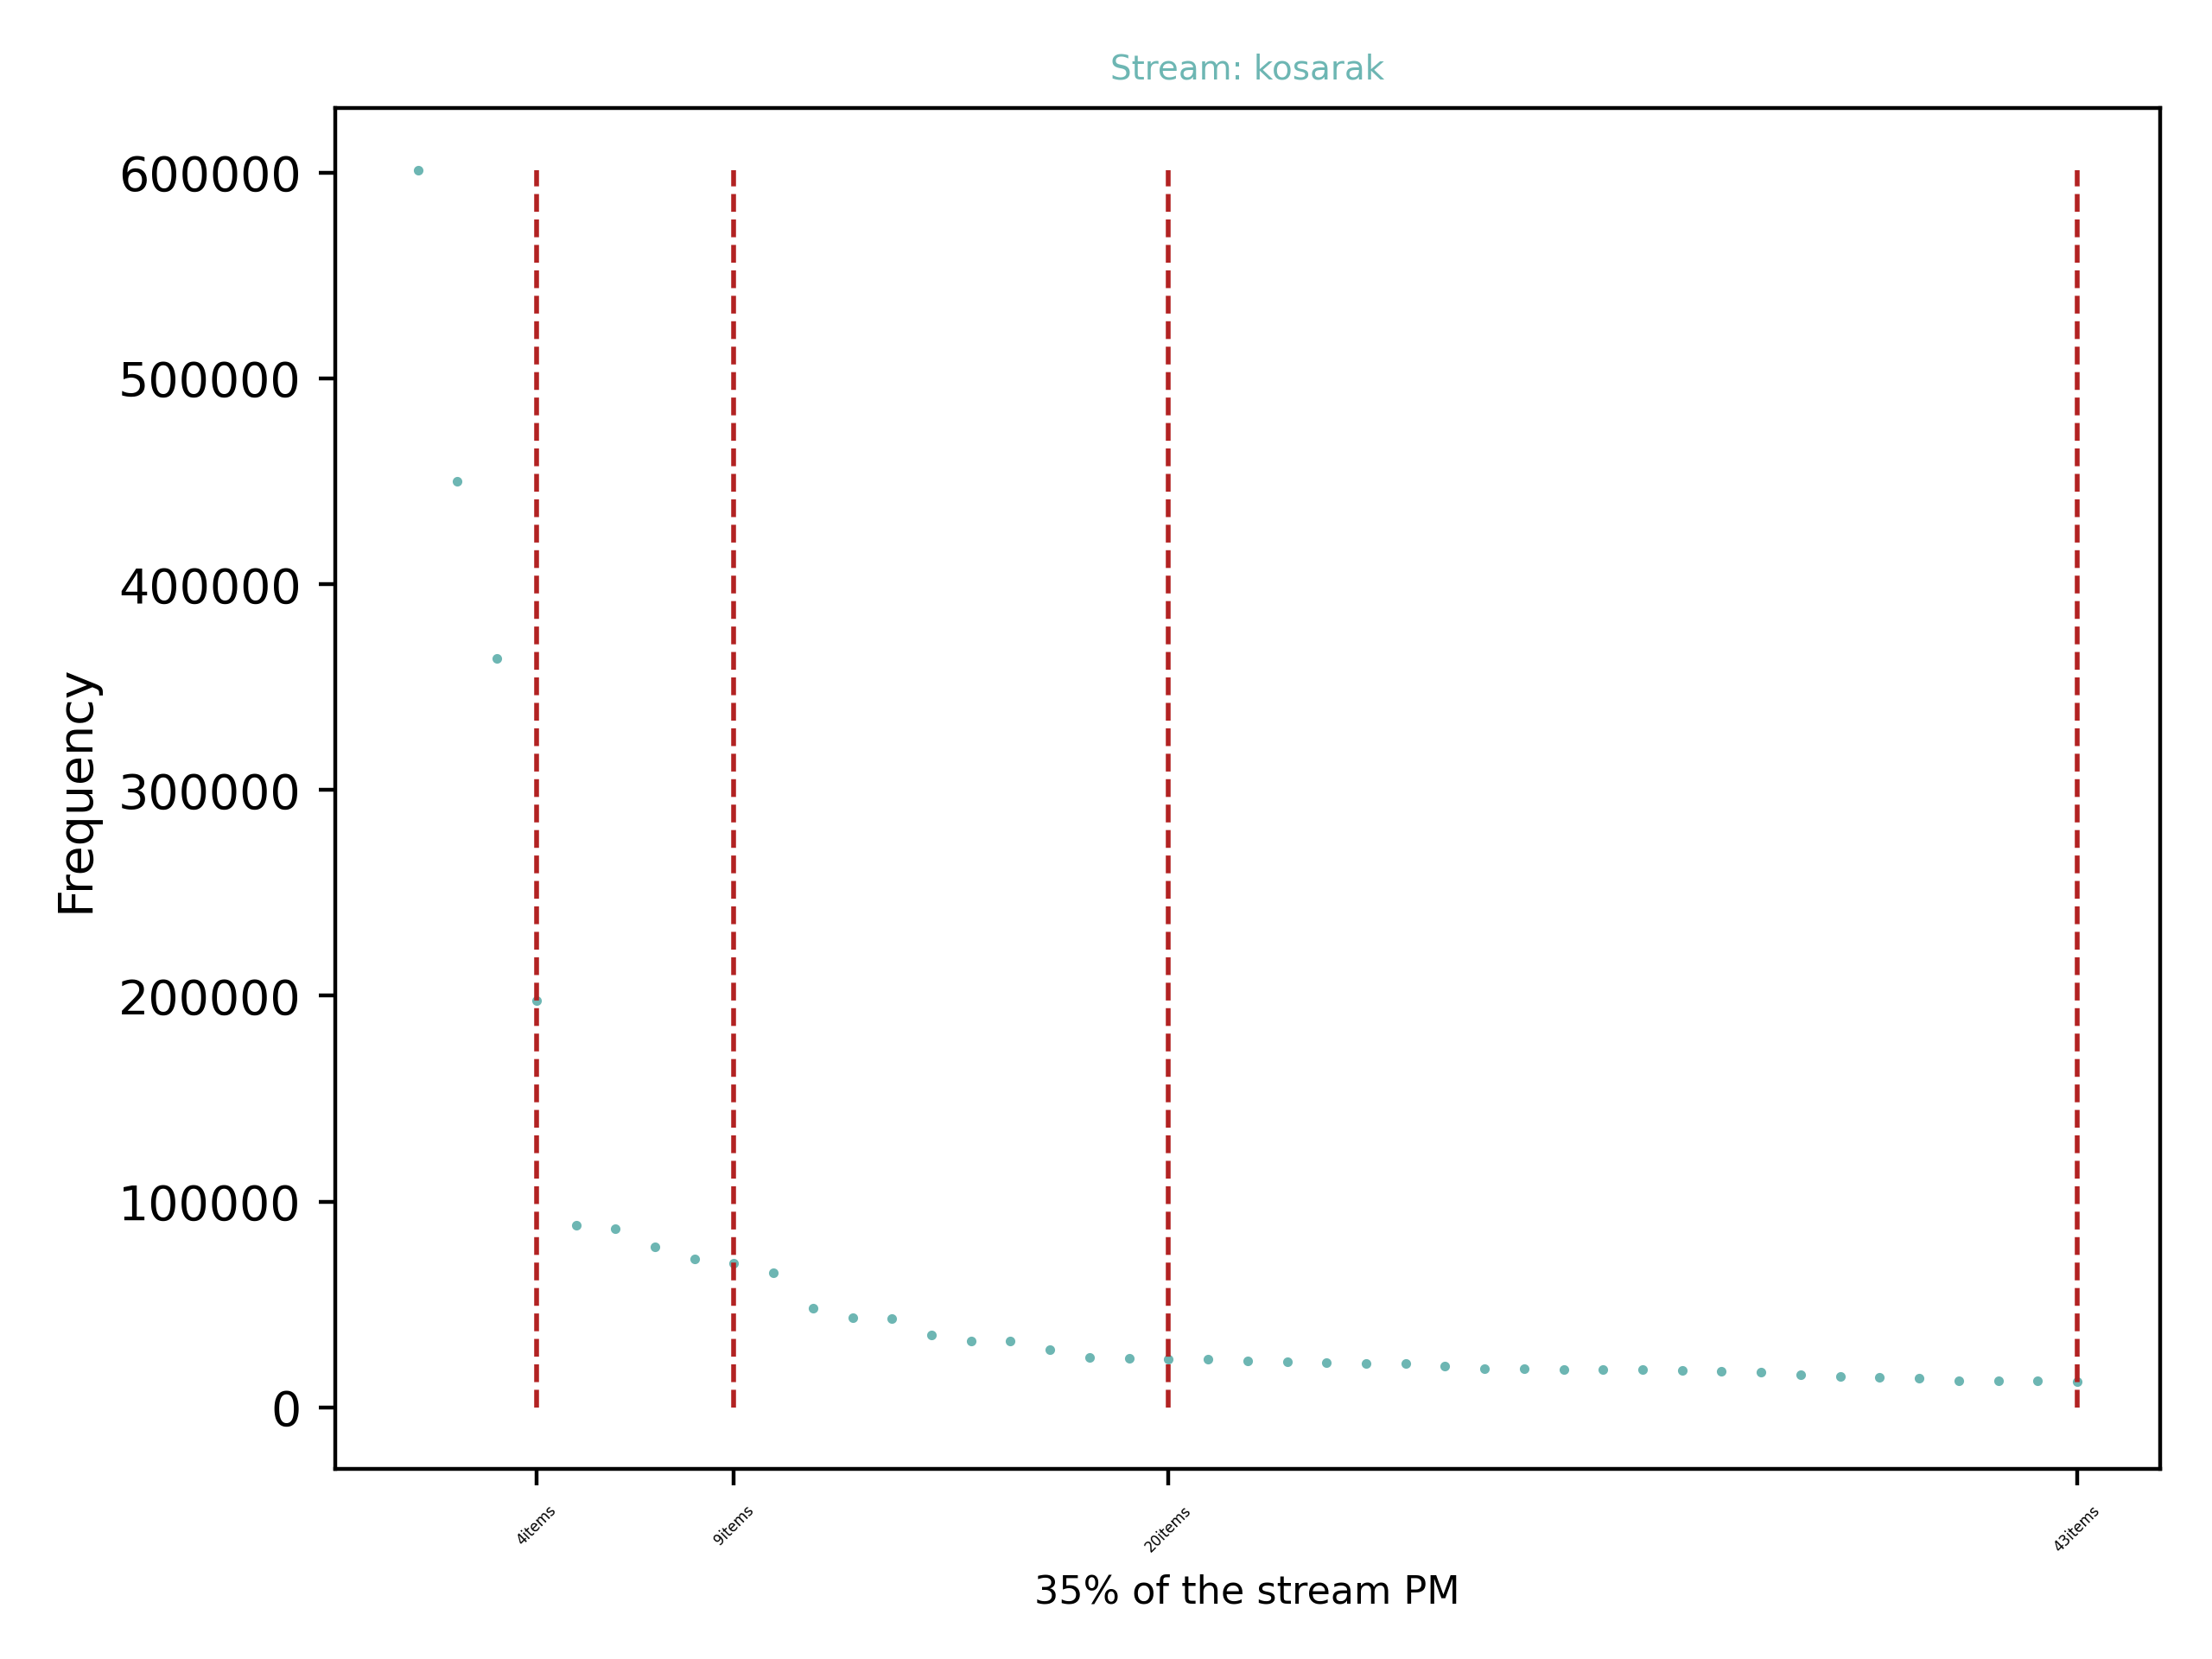
\includegraphics[width=\linewidth]{chapters/ch3_cfe/images/kosarak_pm.png}
    \caption*{Kosarak stream}
  \endminipage\hfill
  \minipage{0.32\textwidth}
    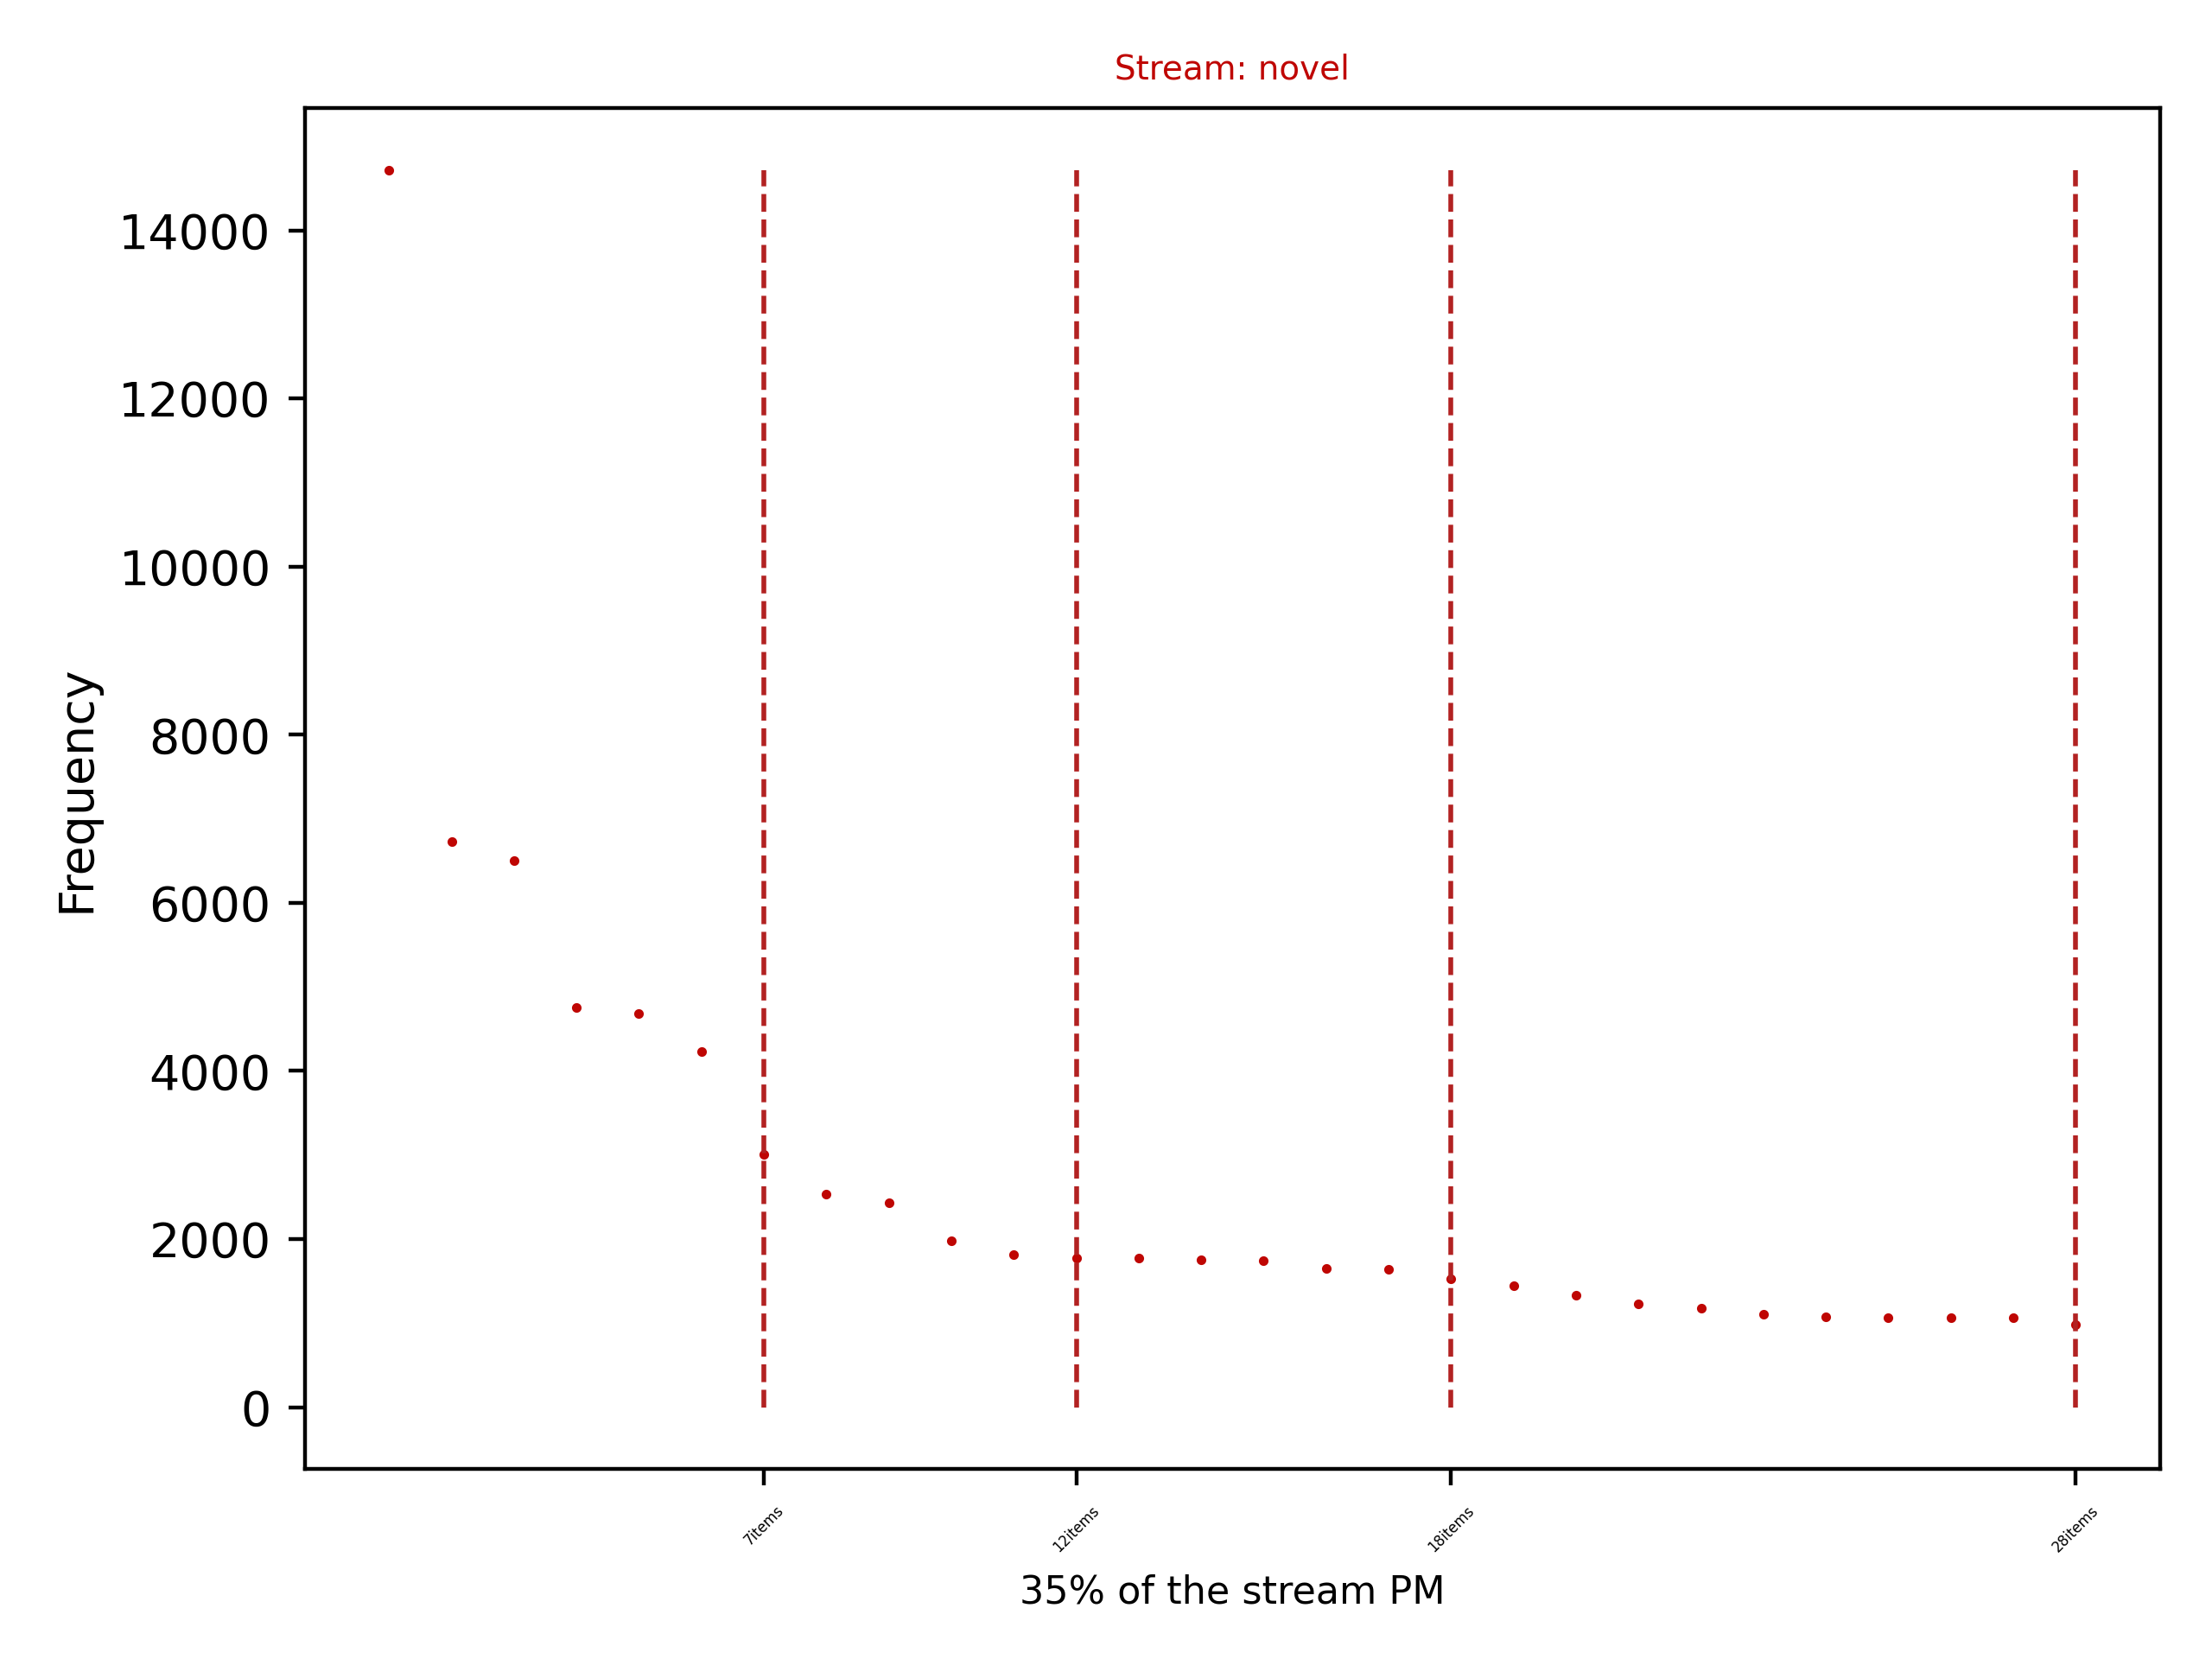
\includegraphics[width=\linewidth]{chapters/ch3_cfe/images/novel_pm.png}
    \caption*{Novel stream}
  \endminipage\hfill
  \minipage{0.32\textwidth}%
    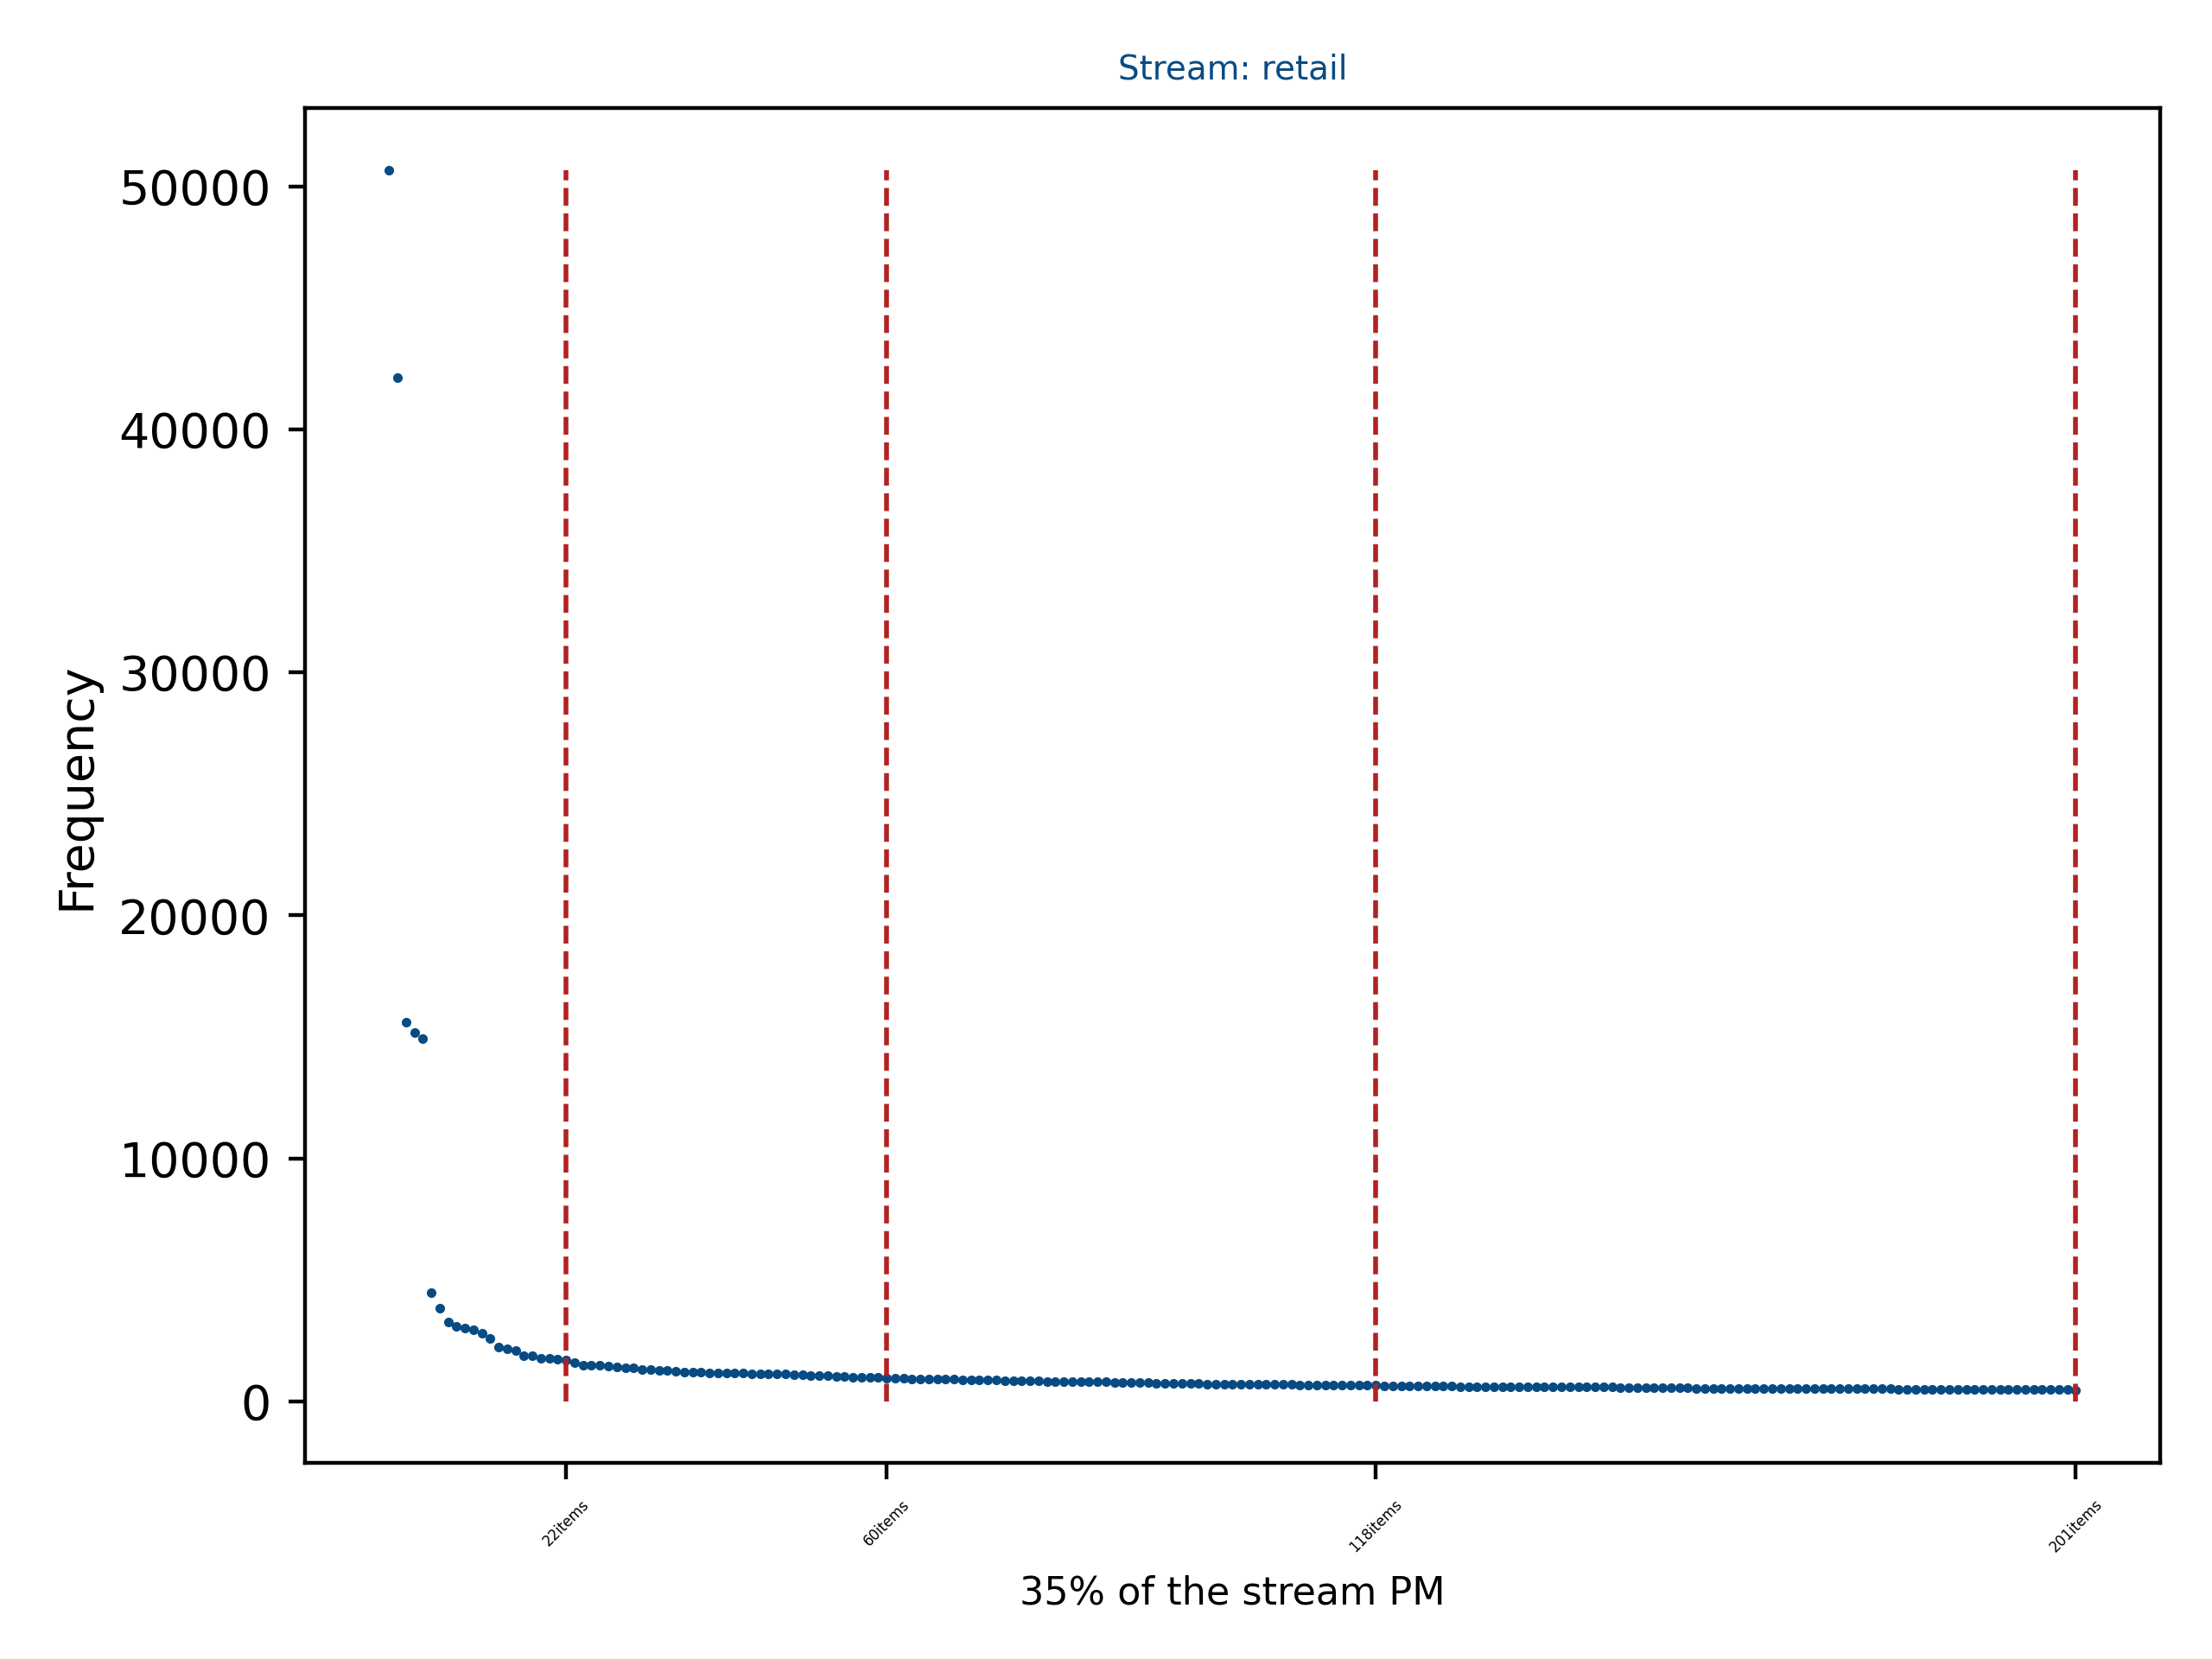
\includegraphics[width=\linewidth]{chapters/ch3_cfe/images/retail_pm.png}
    \caption*{Retail stream}
  \endminipage
  \caption[Stream Frequent Elements.]{We plot the top~$35\%$ probability mass for each stream. That is the most frequent elements that make up~$35\%$ of the total weight of the stream (i.e. the fewest number of elements in each stream whose frequencies sum to such that when divided by the total length of the stream equal~$35\%$). The first vertical red line in each plot is the top~$20\%$ probability mass, the second the top~$25\%$, the third the top~$30\%$, and the last the top~$35\%$. From visual inspection we decided to make the top-$K$ cut-off at, $20$ for Kosarak stream, $22$ for the Novel stream, and~$22$ for the Retail stream.}
  \label{fig:stream_pm} 
\end{figure*}
\paragraph{Measures and Metrics} We want to measure the performance of the CFEs of interest in the non-adversarial setting by determining how well they are able to identify and characterize the heavy elements in the streams above. %\mia{Why is it satisfactory to do it that way - aka test the streams only on limited number of streams? (if not addressed before)}

This problem, with varying but related definitions, is referred to in the literature as the heavy-hitters problem, the hot-items problem, or the top-$K$ problem. 

%\mia{[style] I think the sentence can be written better. 'to apply' - what do we actually mean by that? Can we be more concrete when giving the definition- possibly giving a bit more math-looking one as we have for some other stuff OR reference to a paper with it? }
The simplest of these definitions to apply is that of the top-$K$ problem, which is to simply report the set of elements with the~$K$ highest frequencies (for some~$K$) for a given stream. That is given elements of a stream~$\streamvar{S} \subseteq  \{ e_1,e_2,\ldots,e_M \}$ with associated frequencies~$(n_{e_1},n_{e_2},\ldots,n_{e_M})$ we can order the elements~$\{ e^{*}_{1},e^{*}_{2},\ldots,e^{*}_{M} \}$ such that~$(n^{*}_{e_1} \geq n^{*}_{e_2} \geq \ldots \geq n^{*}_{e_M})$. Then for some~$K \in \mathbb{Z}^{+}$ we output the set of elements~$\{ e^{*}_{1},e^{*}_{2},\ldots,e^{*}_{K} \}$ with the~$K$ highest frequencies~$(n^{*}_{e_1} \geq n^{*}_{e_2} \geq \ldots \geq n^{*}_{e_K})$.

The top-$K$ problem can be solved exactly given space linear to that of the stream by keeping an individual counter for each distinct element in the stream. It is not possible to solve exactly with space less than linear (see~\cite{Roughgarden_Valiant} for a formal impossibility argument), but it is a common technique to place a small data structure such as a min-heap restricted to size~$K$ on top of a CFE and by updating this small structure on each insertion once, one is able to approximate this top-$K$ set~\cite{yang2019heavykeeper,mandal2018topkapi,metwally2006}.

%\mia{How do we know this? Is it a common knowledge for CFE ppl - if so state it as such and give your source for the info.}. 

For our purposes we simply compute the approximate top-$K$ by processing the stream with a compact frequency estimator, querying on every distinct element in the stream, and ordering elements by approximated frequency. Likewise, we compute a true top-$K$ for each stream by processing said stream with a map linear in the size of the stream, computing a frequency for each element, and ordering by true frequency.  We note that we would have achieved identical results by putting a min-heap on top of each structure with fixed sized~$K$, updating as described in~\cite{yang2019heavykeeper} and outputting its contents once the entire stream has been processed. However, for experimental purposes our approach is more extensible than the one that would be used in practice.

%\mia{why don't we also consider the heap - this is possibly tom todo, why the alternative approach, what are its strengths (and weaknesses). How do we justify accepting the weaknesses?}

The number of heavy elements, or perhaps the number of heavy elements one would care about, varies depending on the stream and the application. For instance, it is noted that in a telecommunications scenario when monitoring the top outgoing call destinations of a customer typically a value of~$K$ in the range of~$10-20$ is appropriate~\cite{homen2010}. Moreover, when identifying the most frequent elements of interest of Zipfian distribution it is often of interest to vary~$K$ based on the parameters of the underlying distribution~\cite{charikar2002finding}.

We select~$K$ for each stream by observing the number of clearly identifiable outliers in the underlying stream.  We do this by visually inspecting the selected streams' frequency plots. We set the $x$-axis to enumerate all distinct elements in a stream, ordered from  most to least frequent and the $y$-axis as those distinct elements' corresponding frequencies. We make a cut-off around the point where the frequencies went from very peaked (distinct with prominent frequency jumps from element to element) to flat (many elements with about the same frequency -- the point at which the frequency differences decline less sharply). These frequency plots can be seen in Figure~\ref{fig:stream_pm}. We set~$K=20$ for the Kosarak stream,~$K=22$ for the novel stream, and~$K=22$ for the retail stream. 

We measure the accuracy of the non-adversarial performance according to four different metrics.

\begin{enumerate}[wide, labelwidth=!, labelindent=0pt]
    \item \textbf{Set Intersection Size (SIS):} This measures the size of the set intersection of the true top-$K$ set~$\set{K}$ of the stream and the estimated top-$K$ set~$\tilde{\set{K}}$ as reported by the CFE:~$\text{SIS} = |\set{K} \cap \tilde{\set{K}}|$. This is measure of precision on the estimated top-$K$ set as compared to the true top-$K$ set. A SIS of~$K$ would imply perfect precision. 
    
    \item \textbf{Jaccard Index (JI):} The JI is a statistic that measures the similarity of two sets~\cite{real1996probabilistic}. We use the statistic to determine the similarity of the true top-$K$ set~$\set{K}$ of the stream and the estimated top-$K$ set~$\tilde{\set{K}}$ as reported by the CFE. It is defined as~$\mathrm{JI} = \frac{|\set{K} \cap \tilde{\set{K}}|}{|\set{K} \cup \tilde{\set{K}}|}$. A JI can be in the range~$[0,1]$, with a JI of~$1$ implying a perfect characterization of the true top-$K$ set by the CFE in its top-$K$ estimation. 
    
    \item \textbf{Minimal Top-$\tilde{K}$ to Capture True Top-K (MCT):} 
    This measures determines the minimal size~$L \geq K$ the estimated top-k set~$\tilde{\set{K}}$ would need to be to capture all elements contained in the true top-$K$ set~$\set{K}$. That is if one were to order the frequency estimates of all items made by a particular CFE, we would determine the number of items one would need to examine (starting from the most-frequent going down to the least-frequent) until all the elements from~$\set{K}$ were contained in that ordered set. Thus,~$L-K$ indicates the number of elements that fall out of~$\set{K}$ that are incorrectly being individually estimated to be greater than at least one element that is truly in~$\set{K}$. 
    
    \item \textbf{Average Relative Error on Top-k  elements (ARE)}:
    Average Relative Error is a standard measure to use when comparing CFEs~\cite{yang2019heavykeeper}. It is defined as~$\mathrm{ARE} = \frac{1}{K} \sum_{i=1}^{K} \frac{| \hat{n_{i}} - n_{i}|}{n_{i}}$
    where $i \in [K]$ indexes the true top-$K$ elements for a particular stream.
\end{enumerate}

\paragraph{Results} We crafted reference implementations for all three CFEs of interest: CMS, HK, and CK\footnote{Source code is available at: \url{https://github.com/smarky7CD/cfe-in-adv-envs}}. They are implemented in Python3 and use the BLAKE2b cryptographic hash function %(a 64-bit output hash) 
for independent row hash functions and for a fingerprint hash function in the case of CK and HK. %\mia{How big are fps and cnts? Or is it a parameter that a person running our implementation can vary?} \smnote{Technically, unbounded due to Python, but all remain under 32 bits in size in practice .}

We are interested in comparing performance when the space used by the structures is held constant. Observe that CK is three times as large as  CMS, and HK is twice as large as CMS assuming the same space is used for a counter bucket and a fingerprint bucket (in the CK and HK) across all structures. In practice these buckets could be (say)~$32$-bits. We picked two sets of parameters, a \emph{standard} set and a \emph{constrained} set to test.

The standard set of parameters set~$m=2048,k=4$ for CMS,~$m=1024,k=4$ for HK, and~$m=910,k=3$ for CK. This corresponds to~$32.76$~kB of space when using a 32-bit bucket sizes. We experimentally show that at this size all the structures are able to identify the heavy elements of the streams we test upon with minimal to no error. 

The constrained set of parameters sets~$m=512,k=4$ for CMS,~$m=256,k=4$ for HK, and~$m=341,k=2$ for CK. This corresponds to just~$8.19$~kB of space when using a 32-bit counter and fingerprint bucket sizes. In this space constrained setting the structures are still able to identify the heavy elements of the streams we test upon, but with some degree of moderate error. 

For HK, we set~$d=0.9$ for all experiments, as this is the default chosen by Redis~\cite{redisbloom} and satisfies the desired properties of the exponential decay function stated in~\cite{yang2019heavykeeper}. 

We ran~$1000$ trials for each structure, stream, and parameter triplet using our reference implementations. We randomize each trial on the particular choice of hash functions used for the rows (by selecting a random per-trial seed), as well as the order in which the items in the stream are processed. The latter simulates an item being randomly drawn from the underlying distribution of the stream. We averaged our four metrics for each structure, stream and parameter triplet over the~$1000$ trials. 

\begin{table*}[!ht]
  \centering
  \begin{tabular}{|ccccccc|}
  \hline
  \multicolumn{1}{|c|}{\textbf{Structure}} & \multicolumn{1}{c|}{\textbf{\begin{tabular}[c]{@{}c@{}}Parameters\\ (m,k)\end{tabular}}} & \multicolumn{1}{c|}{\textbf{Stream}}                                                                   & \multicolumn{1}{c|}{\textbf{SIS}}                                                     & \multicolumn{1}{c|}{\textbf{JI}}                                                   & \multicolumn{1}{c|}{\textbf{MCT}}                                                      & \textbf{ARE}                                                  \\ \hline
  \multicolumn{7}{|l|}{\textit{Standard}}                                                                                                                                                                                                                                                                                                                                                                                                                                                                                                                                               \\ \hline
  \multicolumn{1}{|c|}{CK}                 & \multicolumn{1}{c|}{(910,3)}                                                             & \multicolumn{1}{c|}{\multirow{3}{*}{\begin{tabular}[c]{@{}c@{}}Kosarak~($K=20$)\\ Novel~($K=22$)\\ Retail~($K=22$)\end{tabular}}} & \multicolumn{1}{c|}{\begin{tabular}[c]{@{}c@{}}20\\ 22\\ 22\end{tabular}}             & \multicolumn{1}{c|}{\begin{tabular}[c]{@{}c@{}}1\\ 1\\ 1\end{tabular}}             & \multicolumn{1}{r|}{\begin{tabular}[c]{@{}r@{}}20\\ 22\\ 22\end{tabular}}              & \begin{tabular}[c]{@{}c@{}}$\approx 0$\\ $\approx 0$\\ $\approx 0$\end{tabular}             \\ \cline{1-2} \cline{4-7} 
  \multicolumn{1}{|c|}{CMS}                & \multicolumn{1}{c|}{(2048,4)}                                                            & \multicolumn{1}{c|}{}                                                                                  & \multicolumn{1}{c|}{\begin{tabular}[c]{@{}c@{}}19.303\\ 22.999\\ 21.643\end{tabular}} & \multicolumn{1}{c|}{\begin{tabular}[c]{@{}c@{}}0.934\\ 0.999\\ 0.997\end{tabular}} & \multicolumn{1}{r|}{\begin{tabular}[c]{@{}r@{}}20.901\\ 22.001\\ 22.405\end{tabular}}  & \begin{tabular}[c]{@{}c@{}}0.017\\ 0.009\\ 0.040\end{tabular} \\ \cline{1-2} \cline{4-7} 
  \multicolumn{1}{|c|}{HK}                 & \multicolumn{1}{c|}{(1024,4)}                                                            & \multicolumn{1}{c|}{}                                                                                  & \multicolumn{1}{c|}{\begin{tabular}[c]{@{}c@{}}20\\ 22\\ 22\end{tabular}}             & \multicolumn{1}{c|}{\begin{tabular}[c]{@{}c@{}}1\\ 1\\ 1\end{tabular}}             & \multicolumn{1}{r|}{\begin{tabular}[c]{@{}r@{}}20\\ 22\\ 22\end{tabular}}              & \begin{tabular}[c]{@{}c@{}}$\approx 0$\\ $\approx 0$\\ $\approx 0$\end{tabular}             \\ \hline
  \multicolumn{7}{|l|}{\textit{Constrained}}                                                                                                                                                                                                                                                                                                                                                                                                                                                                                                                                               \\ \hline
  \multicolumn{1}{|c|}{CK}                 & \multicolumn{1}{c|}{(341,2)}                                                             & \multicolumn{1}{c|}{\multirow{3}{*}{\begin{tabular}[c]{@{}c@{}}Kosarak~($K=20$)\\ Novel~($K=22$)\\ Retail~($K=22$)\end{tabular}}} & \multicolumn{1}{c|}{\begin{tabular}[c]{@{}c@{}}17.189\\ 21.617\\ 13.442\end{tabular}} & \multicolumn{1}{c|}{\begin{tabular}[c]{@{}c@{}}0.757\\ 0.967\\ 0.441\end{tabular}} & \multicolumn{1}{c|}{\begin{tabular}[c]{@{}c@{}}28.695\\ 22.451\\ 209.439\end{tabular}} & \begin{tabular}[c]{@{}c@{}}$\approx 0$\\ $\approx 0$\\ 0.021\end{tabular}         \\ \cline{1-2} \cline{4-7} 
  \multicolumn{1}{|c|}{CMS}                & \multicolumn{1}{c|}{(512,4)}                                                             & \multicolumn{1}{c|}{}                                                                                  & \multicolumn{1}{c|}{\begin{tabular}[c]{@{}c@{}}18.241\\ 21.638\\ 18.745\end{tabular}} & \multicolumn{1}{c|}{\begin{tabular}[c]{@{}c@{}}0.841\\ 0.969\\ 0.745\end{tabular}} & \multicolumn{1}{c|}{\begin{tabular}[c]{@{}c@{}}24.567\\ 22.473\\ 41.609\end{tabular}}  & \begin{tabular}[c]{@{}c@{}}0.125\\ 0.062\\ 0.296\end{tabular} \\ \cline{1-2} \cline{4-7} 
  \multicolumn{1}{|c|}{HK}                 & \multicolumn{1}{c|}{(256,4)}                                                             & \multicolumn{1}{c|}{}                                                                                  & \multicolumn{1}{c|}{\begin{tabular}[c]{@{}c@{}}20\\ 22\\ 21.976\end{tabular}}         & \multicolumn{1}{c|}{\begin{tabular}[c]{@{}c@{}}1\\ 1\\ 0.998\end{tabular}}         & \multicolumn{1}{c|}{\begin{tabular}[c]{@{}c@{}}20\\ 22\\ 55.008\end{tabular}}          & \begin{tabular}[c]{@{}c@{}} $\approx 0$\\ 0.001\\ 0.005\end{tabular}     \\ \hline
  \end{tabular}
  \caption[Non-adversarial CFE Results.]{A summary of non-adversarial setting results between the CK, CMS, and HK compact frequency estimators.}
  \label{tab:hon-exp-res}
  \end{table*}


We present a summary of the results in Table~\ref{tab:hon-exp-res}. For the \emph{standard} parameter set we see that CK and HK perform best, being able to perfectly capture the true top-$K$ set for each stream with their outputted estimated top-$K$ set in \emph{every} trial. This is indicated by the SIS and MCT being equal to~$K$ and the JI being equal to~$1$ for each stream. Moreover, the estimates on these top-$K$ elements for both of these structures were very tight. The ARE over all trials and streams was~$0$ (ignoring a small rounding error). This indicates that CK and HK nearly perfectly individually estimated every single element in the true top-$K$ across all trials. 
  
CMS with the standard parameter sizing performs almost as well. Only failing to capture the true top-$K$ set with its estimated set a few number of times over the~$1000$ trials. This is indicated by the SIS and MCT being very close to~$K$ and the JI being very close to~$1$ for each stream. However, CMS, as it is prone to overestimation on every element, has slightly higher ARE than the other structures. 

The \emph{constrained} set of parameters presents a challenge for all the CFEs in computing individual frequency estimations on elements in the streams, and as a result computing an accurate estimated top-$K$. This setting only allocates CK a measly~$642$ individual counters to compactly represent streams that all have over~$19,000$ distinct elements. Under these conditions, HK performs best according to our metrics. It perfectly captures the true top-$K$ in both the Kosarak and Novel stream, while only failing to do so in a handful of trials with the Retail stream. Moreover, the ARE is small across all streams -- comparatively less than CMS with the standard parameters. HK by design prioritizes providing accurate estimates on the most frequent elements, by way of its probabilistic decay mechanism. So while it performs well on this task, it severely underestimates middling and low frequency elements at this sizing, reporting an individual frequency estimate very near~$0$ for any element that is not heavy. %This behavior is what we exploit in our attacks to create error in the structure, effectively masking true heavy elements. 

 CMS and CK perform less well in this small space allocation setting. While CMS performs slightly better in capturing the true top-$K$ set within its estimated top-$K$ set, CK continues to give better accuracy on individual point estimations of the true top-$K$ elements across streams due to its internal sub-estimators that provide tighter estimations than CMS.

We observe in this constrained space setting across the structures measured performance is the worst on the Retail stream. This is because the Retail stream has a flatter distribution as compared to the other streams. That is to say, it has very few clearly identifiable heavy elements before containing a large collection of elements of about the same frequency. This can be seen in the frequency plot in Figure~\ref{fig:stream_pm}. The Retail element with frequency rank~$22$ has a true frequency of~$1715$ while the Retail element of frequency rank~$56$ has a true frequency of~$1005$. Comparing this to $n_{22} = 22631, n_{56} = 9559$ and~$n_{22} = 1176, n_{56} = 474$, respectively for the Kosarak and Novel stream, one can see that the relative fall off in true frequency is far less pronounced within this region of the Retail stream. This in turn leads to small errors in the individual frequency estimations of elements near (but outside) the true top-$K$ of the Retail stream propagating to the top-$K$ estimation -- by making it challenging for the CFEs to draw a clear distinction between the truly heavy elements and the nearly heavy elements. The upshot being, one needs larger structures to accurately estimate these flatter streams.

In sum, CK performs comparatively well to both CMS and HK in this particular task. In fact, CK performed better than CMS when not burdened with \emph{very} tiny space constraints. It is able to perfectly estimate the true top-$K$ for all streams over all trials with only $2730$ individual counters in the standard parameter setting, while also being adversarial robust where the others structures are not. 



\subsection{Attacks Against the CK}\label{sub-sec:ck-attacks}
Our attacks against CK are almost one-to-one with those we present against the CMS with one major difference. Recall from Corollary~\ref{cor:fx:MA:Theta13:nx} that if at least one counter in some row~$i$ of the element~$x$ we are querying on maps to has~$|V^i_x| \leq 1$ then CK returns estimate~$\hat{n}_x$ such that~$\hat{n}_x = n_x$, i.e. $\CK(x)$ is a perfect estimate of~$x$. This implies that for an error to exist in a frequency estimation of~$x$ it must be that~$\forall i \in [k]$ it is necessary that~$|V^i_x| \geq 2$. In the attack setting this means we need to find a $2$-cover (specifically a~$(\set{FP}_{x},x,2)$-cover) on~$x$ to create error.

A 2-cover~$\set{C}$ for~$x$ contains elements~$\{y_1,y_2,\ldots,y_t\}$ such that for every counter $x$ maps to in positions~$(p_1,p_2,\ldots,p_k) \gets R(K,x)$ it is such that at least two distinct elements in~$\set{C}$ cover each counter. In our attack model we assume an initially empty representation and we never insert~$x$ in any of our attacks (except for once to discover its counter positions in the public representation, private hash setting). 

We attack CK in a two-step process, as with CMS and HK. We first find a 2-cover for our target element~$x$ and then repeatedly insert the 2-cover to create error. Under the assumption that~$x$ does not own any of its counters in the~$A$ substructure of the CK (which is guaranteed in our attack model\footnote{Save for the trivial case in the public representation, private hash setting when no cover is able to be found.}), then the~$\Theta_1$ sub-estimator will be used to make the final error evaluation~$\QRYO$ query on~$x$. Say that after some process of finding a 2-cover for~$x$ (which will be of size~$\leq 2k$ -- for this discussion we will assume the size of the 2-cover is exactly~$2k$) we have~$\omega$ insertions to repeatedly insert the elements in the cover. Repeated and equal insertions of each of the elements in the 2-cover for~$x$ will cause the values in all of $x$'s counters in the~$M$ substructure of the CK to be of value~$\frac{\omega}{k}$. In the~$A$ substructure the value in the counters that~$x$ maps to will have value~$1$ and be owned by some element in the 2-cover. This is because (under the no-fingerprint collision assumption) in the initially empty structure, ownership of said counters will flip-flop on each iteration of the insertions of the 2-cover between the two distinct elements that map to these counters in accordance with the~$\Up$ algorithm of the HK with~$d=1$. 

Then applying the estimation from~$\Theta_1$ we see that we will generate error on~$x$ equal to~$\frac{\omega}{2k}$. If we hold~$k$ constant and assume that we are attacking a CMS under the same conditions (we have found a 1-cover for a target~$x$ through some process and have~$\omega$ insertions to accrue error) we will have an error of~$\frac{\omega}{k}$, which is twice that of the CK under the same conditions. Under the same assumptions for HK, in addition to the assumption that we have already locked-down the counters of the target with initial insertions of the cover in the structure, we will achieve an error on the target of~$\omega$ -- which is~$\omega - \frac{\omega}{2k}$ greater than that of the CK. We will see this pattern holds when giving concrete experimental attack error results at the conclusion of this section.

\paragraph{Public hash and representation setting}
\begin{figure*}[ht!]
	\Wider[2em]{
		\centering
		\begin{pchstack}[boxed,center,space=0.4em]
			\procedure[linenumbering, headlinecmd={\vspace{.1em}\hrule\vspace{.2em}}]{$\text{CoverAttack}^{\HASHO,\UPO,\QRYO}(x, K, {\repr})$}{%
				\textrm{cover} \, {\gets} \textrm{FindCover}^{\HASHO}(2,x,K)\\
				\pcuntil q_U \ \UPO \text{-queries made:}\\
				\t \pcfor e \in \textrm{cover}{:} \ \UPO(e)\\
				\pcreturn \textrm{done}
			}
			\procedure[linenumbering, headlinecmd={\vspace{.1em}\hrule\vspace{.2em}}]{$\text{FindCover}^{\HASHO}(r, x, K)$}{%
				\textrm{cover} \gets \emptyset; \,
				\textrm{found} \gets \mathsf{False}\\
				\set{I} \gets \emptyset; \,\textrm{tracker} \gets \zeros(k)\\
				\hspace{-.5em}
				\pcgraycomment{$R(K,x)[i]=\HASHO(\encode{i,K,x})$}\\
				(p_1,p_2,\ldots,p_k) \gets R(K,x)\\
				\pcwhile \textrm{not found}\\
				\t \pcif q_H \ \HASHO\text{-queries made}\\
				\t \t \pcreturn \emptyset\\
				\t y \getsr \set{U}\setminus (\set{I} \cup \{x\})\\
				\t \set{I} \gets \set{I} \cup \{y\}\\
				\t (q_1,q_2,\ldots,q_k) \gets R(K,y)\\
				\t \pcfor i \in [k]\\
				\t \t \pcif p_i = q_i~\textbf{and}~\textrm{tracker}[i] < r\\
				\t \t \t \textrm{cover} \gets \textrm{cover} \cup \{y\}\\
				\t \t \t \textrm{tracker}[i]~+= 1\\
				\t \pcif \mathsf{sum}(\textrm{tracker}) = rk\\
				\t \t \textrm{found} \gets \mathsf{True}\\
				\pcreturn \textrm{cover}
			}
		\end{pchstack}
	}
	\caption{Cover Set Attack for the CK in public
		hash function setting. 
%		We use $R(K,x)$ to mean $(\HASHO(\encode{1,K,x}),\HASHO(\encode{2,K,x},\ldots,\HASHO(\encode{k,K,x})))$.
		The attack is parametrized with  the update and $\HASHO$ query budget $q_U$ and $q_H$.
	}
%\mia{The attck is 1-1 with CMS attack (Figure \ref{fig:attack-cms-hfcs}) with $\textrm{FindCover}^{\HASHO}(1,x,K)$ changing to $\textrm{FindCover}^{\HASHO}(2,x,K)$ (first line of the code)! So, I think that we do NOT need this code in the paper.}
	\label{fig:attack-ck-hf2cs}
\end{figure*}
As our other attacks (for CMS and HK) in this setting, the CK attack (Figure~\ref{fig:attack-ck-hf2cs}) can be viewed as a two-step process.  In this setting, we find a 2-cover for target~$x$ using the $\HASHO$ oracle only, and then accumulate error for the target by repeatedly inserting the 2-cover. Each insertion of the 2-cover increases the error by one. The two cover can be inserted at least $\frac{q_U}{2k}$ as the size of the cover is~$\leq 2k$.
We apply the same analysis used for the CMS attack, but replace $k(1 + L^1)$ with $k(1 + L^2)$ as the number of $\HASHO$-queries to complete the cover-finding step, as again, we now find a 2-cover. Assuming $q_U > 2k$ (so that any found $\set{C}$ can be inserted at least once)
we arrive at
%\begin{align}\label{eqn:pub-pub-pr-cover-qH-CK}
$\mathbb{E}[\rverr] \geq \left\lfloor\frac{q_U}{2k}\right\rfloor \Pr\left[L^2 \leq \frac{q_H-k}{k}\right]$
%\end{align}
Using results from Section \ref{sec:cov-set} we can further obtain a concrete expression for $\Pr\left[L^2 \leq \frac{q_H-k}{k}\right]$. 

\paragraph{Private hash and representation setting}
\begin{figure*}[ht!]
	%\Wider[2em]{
		\centering
		\begin{pchstack}[boxed,center,space=0.5em]
		\begin{pcvstack}[space = 0.45em]
	\procedure[linenumbering, headlinecmd={\vspace{.1em}\hrule\vspace{.2em}}]{$\text{CoverAttack}^{\UPO,\QRYO}(x, \bot, \bot)$}{%
		\textrm{cover} \gets \textrm{FindCover}^{\UPO,\QRYO}( x)\\
		\pcuntil q_U \ \UPO \text{-queries made:}\\
		\t \pcfor e \in \textrm{cover}{:} \ \UPO(e)\\
		\pcreturn \textrm{done}
	}
	\procedure[linenumbering, headlinecmd={\vspace{.1em}\hrule\vspace{.2em}}]{$\text{MinUncover}^{\UPO,\QRYO}(x, a', \text{cover})$}{%
		b' \gets a' - 1\\
		\pcwhile a' \not= b'\\
		\t \pcif (q_U-|\textrm{cover}| + 1)\UPO\text{-} \\
		\t \t \text{ or } q_Q \ \QRYO\text{-queries made:}\\
		\t \t \t \pcreturn \textrm{cover}\\
		\t b' \gets a'\\
		\t \pcfor y \in \text{cover}: \UPO(y)\\
		\t a' \gets \QRYO(x)\\
		\pcreturn a'
	}
\end{pcvstack}
\procedure[linenumbering, headlinecmd={\vspace{.1em}\hrule\vspace{.2em}}]{$\text{FindCover}^{\UPO,\QRYO}(x)$}{%
	\pcgraycomment{find $2$- cover for x}\\
	\textrm{cover} \gets \emptyset\\
	\textrm{found} \gets \mathsf{False}\\
	%			; \textrm{lessened} \gets \mathsf{False}\\
	\set{I} \gets \emptyset; a \gets \QRYO(x) \\
	\hspace{-.5em}
	\pcwhile \textrm{not found} \\
	\t \pcif q_U \ \UPO \text{- or } q_Q \ \QRYO\text{-queries made}\\
	\t \t \pcreturn \textrm{cover}\\
	\t y \getsr \univ \setminus (\set{I} \cup \{x\})\\
	\t \set{I} \gets \set{I} \cup \{y\}\\
	\t \UPO(y); \ a' \gets \QRYO(x)\\
	\t \pcif a' \not= a: \\
	\t \t \textrm{cover} \gets \{y\}\\
	\t \t \textrm{found} \gets \mathsf{True}\\
	\pcfor i \in [2, 3, \dots, 2 \cdot k]\\
	\t a \gets \text{MinUncover}^{\UPO,\QRYO}(x, a', \text{cover}) \\
	\t \pcif a = \textrm{cover}: \pcreturn \textrm{cover}\\
	\t \pcfor y \in \set{I} \ \pcgraycomment{in order of insertion to $\set{I}$}\\
	\t \t \pcif q_U \ \UPO \text{- or } q_Q \ \QRYO\text{-queries made}\\
	\t \t \t \pcreturn \textrm{cover}\\
	\t \t \UPO(y); a' \gets \QRYO(x) \\
	\t \t \pcif a' \not= a: \\
	\t \t \t \textrm{cover} \gets \textrm{cover} \cup \{y\}\\
	%			This is just here so the algorithm is exactly the same for the CK!
	\t \t \t \set{I} \gets \set{I} \setminus \{y\}\\
	\t \t \t \textbf{break}\\
	\pcreturn \textrm{cover} \ \pcgraycomment{cover is inserted at least once}
}
\end{pchstack}
		%}
	\caption{Cover Set Attack for the CK in private
		hash function and representation setting. 
		The attack is parametrized with the update query and query query budget -- $q_U$ and $q_Q$.}
%\mia{The attck is 1-1 with CMS attack (Figure \ref{fig:attack-cms-iqcsa}) with $\textrm{FindCover}^{\UPO,\QRYO}(x)$, line \ref{alg:CMS:CK:change} changing to go up to $2k$! This is because we are now finding a two cover! Overall, I think that we do NOT need this code in the paper.}
%\mia{@Sam I am hesitant to define $\textrm{FindCover}^{\UPO,\QRYO}(x)$ with argument $r$. I do not see if taking the algorithm with $r!=2$ would make any sense for CK (would find $r$ cover, even for $r=4$), or that the algorithm with $r!=1$ actually finds an $r$-cover for CMS.}
%\mia{Is \textrm{FindCover} alg. name collision between the CMS and CK attack too confusing? (irrelevant if we do not have the code in the paper.)}
	\label{fig:attack-ck-iq2csa}
\end{figure*}

Our CK attack for the setting (Figure~\ref{fig:attack-ck-iq2csa}) is essentially the same as the CMS attack, except a 2-cover (as opposed to a 1-cover) is detected and repeatedly inserted to build up the error. Using analysis similar to the CMS case and assuming~$q_Q$ is not the limiting factor,

$$\rverr \geq 
	\left \lfloor \left( \frac{\ell+1}{2} + \frac{1}{\ell}\left(q_U + \sum_{i=1}^{\ell-1}(\ell-i)\delta_i \right) - L^2 \right) \right\rfloor$$

with~$\ell \leq 2k$ rounds to find a 2-cover. The error bound is similar to the one for the CMS attack, but with $L^1$ replaced with $L^2$ as now $|\streamvar{I}|$ is precisely~$L^2$.  

For reasonable sizes of the CK we mainly expect $\ell = 2k$ (for the CMS case we expected $\ell{=}k$) and that $\mathbb{E}\left[\delta_1\right]$ are bounded by a constant that is small relative to $m, q_U/k$. Given that $k \ll m$, we expect the following to approximate $\mathbb{E}[\rverr]$:
\begin{align*}
	&\mathbb{E}\left[\left\lfloor \left( \frac{2k+1}{2} + \frac{1}{2k}\left(q_U + \sum_{i=1}^{2k-1}(2k-i)\delta_i \right) - L^2 \right) \right\rfloor\right]\approx \frac{q_u}{2k} -  \mathbb{E}[L^2].
\end{align*}

\paragraph{Public hash and private representation setting}
As with the CMS, the attack and analysis from the public hash and representation setting applies.

\paragraph{Private hash and public representation setting}
This attack (Figure~\ref{fig:attack-ck-io2csa}) is one-to-one with the CMS attack in the same setting, but again we find 2-cover as opposed to a 1-cover. Hence,
$\mathbb{E}[\rverr] \geq \frac{q_U-1-\mathbb{E}\left[L^2\right]}{2k} \gtrapprox \frac{q_U-1-2mH_k}{2k}.
$
%$
%\mathbb{E}[\rverr] \geq \Pr[L^2 \leq \ell_U - 1] \left(\floor(\frac{q_U-\ell_U}{2k}) + 1\right)
%$
\begin{figure*}[ht!]
	\centering
	\begin{pchstack}[boxed,center, space=0.5em]
		\procedure[linenumbering, headlinecmd={\vspace{.1em}\hrule\vspace{.2em}}]{$\text{CoverAttack}^{\UPO,\QRYO}(x, \bot, \repr)$}{%
			\textrm{cover} \gets \textrm{FindCover}^{\UPO}(2,x, \repr)\\
			\pcuntil q_U \ \UPO \text{-queries made:}\\
			\t \pcfor e \in \textrm{cover}{:} \ \UPO(e)\\
			\pcreturn \textrm{done}
		}
		\procedure[linenumbering, headlinecmd={\vspace{.1em}\hrule\vspace{.2em}}]{$\text{FindCover}^{\UPO}(r, x, \repr)$}{%
			\left<M, A\right> \gets \repr\\
			\textrm{cover} \gets \emptyset; \,
			\textrm{found} \gets \mathsf{False}\\
			\set{I} \gets \emptyset; \,\textrm{tracker} \gets \zeros(k)\\
			\left<M', A'\right> \gets \UPO(x)\\
			\pcgraycomment{compute $x$'s indices}\\
			\pcfor i \in [k] \\
			\t \pcfor  j \in [m]\\
			\t \t \pcif M'[i][j] \not= M[i][j]\\
			\t \t \t  p_i \gets j; \textbf{break};\\
			\hspace{-.5em}
			\pcwhile \textrm{not found}\\
			\t \pcif q_U \ \UPO\text{-queries made}:\pcreturn \emptyset\\
			\t y \getsr \set{U}\setminus (\set{I} \cup \{x\})\\
			\t \set{I} \gets \set{I} \cup \{y\}\\
			\t  \left<M, A\right> \gets \left<M', A'\right> \\
			\t \left<M', A'\right>  \gets \UPO(y) \\
			\t \pcgraycomment{compute $y$'s indices}\\
			\t \pcfor i \in [k] \\
			\t \t \pcfor  j \in [m]\\
			\t \t \t \pcif M'[i][j] \not= M[i][j]\\
			\t \t \t  \t q_i \gets j; \textbf{break};\\
			\t \pcfor i \in [k]\\
			\t \t \pcgraycomment{compare $x$'s and $y$'s indices row by row}\\
			\t \t \pcif p_i = q_i~\textbf{and}~\textrm{tracker}[i] < r\\
			\t \t \t \textrm{cover} \gets \textrm{cover} \cup \{y\}\\
			\t \t \t \textrm{tracker}[i]~+= 1\\
			\t \pcif \mathsf{sum}(\textrm{tracker}) = rk\\
			\t \t \textrm{found} \gets \mathsf{True}\\
			\pcreturn \textrm{cover}
		}
	\end{pchstack}
	\caption{Cover Set Attack for the CK in private
		hash function and public representation setting. 
		The attack is parametrized with  the update query budget $q_U$.
	}
	%\mia{The attck is 1-1 with CMS attack (Figure \ref{fig:attack-cms-iocsa}) with $\textrm{FindCover}^{\UPO,\QRYO}(1,x,\repr=M)$ changing to $\textrm{FindCover}^{\UPO,\QRYO}(2,x,\repr=\left<M,A\right>)$ (first line of the code), and algorithm FindCover only using CMS's part ('half') of the representation to find element's indices (or similarly HK's part of the representation - it is equivalent). So,do we need this code in the paper?}
	\label{fig:attack-ck-io2csa}
\end{figure*}

\paragraph{Attack Comparisons}
\begin{table*}[htb!]
	\centering
	\begin{tabular}{|c|ccc|ccc|}
	\hline
						 & \multicolumn{3}{c|}{\textbf{Public Hash Setting}}                                                                & \multicolumn{3}{c|}{\textbf{\begin{tabular}[c]{@{}c@{}}Private Hash,\\ Private Rep Setting\end{tabular}}}       \\ \hline
	\textbf{Structure}   & \multicolumn{1}{c|}{$|\mathrm{cover}|$} & \multicolumn{1}{c|}{Experimental~$\rverr$} & $\mathbb{E}[\rverr]$ & \multicolumn{1}{c|}{$|\mathrm{cover}|$} & \multicolumn{1}{c|}{Experimental~$\rverr$} & $\mathbb{E}[\rverr]$ \\ \hline
	$\CK,(m=682,k=4)$    & \multicolumn{1}{c|}{$7.96$}             & \multicolumn{1}{c|}{$131821.00$}                & $131072.00$          & \multicolumn{1}{c|}{$7.96$}             & \multicolumn{1}{c|}{$130796.69$}                & $127432.90$          \\ \hline
	$\CMS, (m=2048,k=4)$ & \multicolumn{1}{c|}{$3.99$}             & \multicolumn{1}{c|}{$263017.82$}                & $262144.00$          & \multicolumn{1}{c|}{$3.99$}             & \multicolumn{1}{c|}{$261116.16$}                & $257877.34$         \\ \hline
	$\HK, (m=1024,k=4)$  & \multicolumn{1}{c|}{$3.99$}             & \multicolumn{1}{c|}{$1047502.69$}               & $1047500.00$         & \multicolumn{1}{c|}{$4.0$}              & \multicolumn{1}{c|}{$1038804.55$}               & $1038018.54$        \\ \hline
	$\CK,(m=1365,k=8)$   & \multicolumn{1}{c|}{$15.97$}            & \multicolumn{1}{c|}{$65667.10$}                 & $65536.00$           & \multicolumn{1}{c|}{$15.93$}            & \multicolumn{1}{c|}{$63776.52$}                 & $56618.28$          \\ \hline
	$\CMS, (m=4096,k=8)$ & \multicolumn{1}{c|}{$8.00$}             & \multicolumn{1}{c|}{$131072.00$}                & $131072.00$          & \multicolumn{1}{c|}{$7.99$}             & \multicolumn{1}{c|}{$127029.66$}                & $119939.65$         \\ \hline
	$\HK, (m=2048,k=8)$  & \multicolumn{1}{c|}{$7.96$}             & \multicolumn{1}{c|}{$1046434.76$}               & $1046424.00$         & \multicolumn{1}{c|}{$7.98$}             & \multicolumn{1}{c|}{$1007439.04$}               & $996946.87$         \\ \hline
	\end{tabular}
	\caption{A comparison of~$\rverr$ accumulated by the different structures during attacks in the public hash setting and the private hash, private representation setting. We give the average size of the cover set and average error accumulated in each structure, setting pair over the~$100$ experiment trials. We also give the~$\mathbb{E}[\rverr]$ according to our analysis. }
	\label{tab:attack-comp}
\end{table*}
We implemented our attacks against all structures in all settings to experimentally verify their correctness and our analysis. In Table~\ref{tab:attack-comp} we present a summary of results for the public hash setting (our least restrictive setting) and the private hash, private representation setting (our most restrictive setting.). We experiment on two sets of parameters, one fixing~$k=4$ and the other~$k=8$. We then select a reasonable value of~$m$ for CMS and then half it for HK and third it for CK so that the same space is used in each structure. We fix adversarial resources such that~$q_H,q_U,q_Q = 2^{20}$. In practice this ensures that the number of~$\HASHO$ queries or~$\QRYO$ queries will not be the bottleneck in our attacks and that we are able to generate sufficient error in each attack to showcase overall trends. We run each attack setting and structure pairing over~$100$ trials, selecting a random target in each trial, and average the results. 

Observe the pattern that when holding~$k$ constant and setting reasonable~$m$ values, adjusting such that CMS, CK, and HK use the same space, attacks against CK generate the least amount of error. The attacks against CK produce about half of the amount of error as opposed to the CMS attacks, and about~$q_U - \frac{q_U}{2k}$ less the amount of error as opposed to the HK attacks. Moreover, observe that our analytical results closely match those of our experimental results. 

\subsection{Adversarial Robustness}\label{sub-sec:ck-flags}
%
\begin{figure*}[h]
	\Wider[3em]{
		\centering
		\begin{pcvstack}[boxed,center,space=0.5em]
			\begin{pchstack}
				\begin{pcvstack}[space=0.45em]
					\procedure[linenumbering, headlinecmd={\vspace{.1em}\hrule\vspace{.2em}}]{$\Rep_K(\setS)$}{%
						M \gets \zeros(k,m)\\
%						\pcgraycomment{$k\times m$ (fp,cnt) 2-d array}\\
						\pcfor i \in [k] \\
						\t A[i] \gets [(\star,0)]\times m\\
						\repr \gets \langle M,A\rangle\\
						\pcfor x \in \setS \\
						\t \repr \, {\getsr} \Up_K(\repr,{\up_{x}})\\
						\pcreturn \repr
					}
					\procedure[linenumbering, headlinecmd={\vspace{.1em}\hrule\vspace{.2em}}]{$\Up_K(\repr,\up_x)$}{%
						\langle M,A\rangle \gets \repr\\
						M  \getsr \Up^\CMS_{K}(M ,\up_x)\\
						A \getsr \Up^\HK_{K}(A ,\up_x)\\
						\pcreturn \repr {\gets}  \langle M,A\rangle
					}
				\end{pcvstack}
				\begin{pcvstack}[space=0.45em]
					\procedure[linenumbering, headlinecmd={\vspace{.1em}\hrule\vspace{.2em}}]{$\Qry_K(\repr,\qry_x)$}{%
						\langle M, A \rangle \gets \repr\\
						(p_1,\ldots,p_k) \gets R(K,x), \, \mathrm{fp}_{x} \gets T(K,x)\\
						\Theta_1,\Theta_2,\Delta \gets \infty\\
                        \text{flag} \gets \mathsf{False}\\
                        N \gets \sum_{j=1}^{m} M[1][j]\\
						%\pcgraycomment{CMS only overestimates}\\
						\cnt_{\text{UB},x}\gets \Qry\CMS_{K}(M,\qry_x)\\
						%\pcgraycomment{HK only underestimates}\\
						\cnt_{\text{LB},x} \gets \Qry^\HK_{K}(A,\qry_x)\\
						%\pcgraycomment{return upperbound if equal to lowerbound}\\
						\pcif \cnt_{\text{UB},x} =  \cnt_{\text{LB},x}\\
						\t \pcreturn \cnt_{\text{UB},x},\text{flag}\\
						\pcfor i \in [k] \\
						%\t \pcgraycomment{if never observed}\\
						\t \pcif A[i][p_i].\mathrm{fp} = \star\\
						\t \t \cnt_{\text{UB},x} \gets  0\\
						\t \t \pcreturn 0,\text{flag}\\
						%\t \pcgraycomment{upper bound adjustment}\\
						%\t \pcgraycomment{x does not own counter}\\
						\t \pcelse \pcif A[i][p_i].\mathrm{fp} \not= \fp_x\\
						\t \t \Theta \gets \frac{M[i][p_i] {-} A[i][p_i].\cnt {+}1}{2}\\
						\t \t \Theta_1 {\gets} {\min}\left\{ \Theta_1, \Theta \right\}\\
                        \t \t \hat{\Delta} \gets \frac{M[i][p_i] {-} A[i][p_i].\cnt {+} 1}{2}\\
                        \t \t \Delta {\gets} 
						{\min}\left\{ 
						\Delta, \hat{\Delta}\right\}\\
%						\t \t \Theta_1 {\gets} 
%						{\min}\left\{ 
%						\Theta_1, \frac{M[i][p_i] {-} A[i][p_i].\cnt {+}1}{2}
%						\right\}\\
						%\t \pcgraycomment{x owns counter}\\
						\t \pcelse \pcif A[i][p_i].\mathrm{fp} = \fp_x\\
						\t \t \Theta \gets \frac{M[i][p_i] {+} A[i][p_i].\cnt}{2}\\
						\t \t \Theta_2 {\gets} 
						{\min}\left\{ 
						\Theta_2, \Theta\right\}\\
                        \t \t \hat{\Delta} \gets \frac{M[i][p_i] {-} A[i][p_i].\cnt}{2}\\
                        \t \t \Delta {\gets} 
						{\min}\left\{ 
						\Delta, \hat{\Delta}\right\}\\
%                        \t \t \Theta_2 {\gets} 
%						{\min}\left\{ 
%						\Theta_2, \frac{M[i][p_i] {+} A[i][p_i].\cnt}{2}
%						\right\}\\
						\cnt_{\text{UB},x} {\gets} \floor(\min\left\{ \Theta_1, \Theta_2 \right\}) \\
                        \pcif \Delta \geq \psi N\\
                        \t \text{flag} \gets \mathsf{True}\\
						\pcreturn \cnt_{\text{UB},x}, \text{flag}
					}
				\end{pcvstack}
			\end{pchstack}	
		\end{pcvstack}
	}
	\caption[Robust Flag Raising Count-Keeper Structure.]{Keyed structure $\CK[R,T,m,k,\psi]$ supporting point-queries for any potential stream element~$x$ ($\qry_x$) and the ability to raise a flag on ``bad'' frequency estimation.
		$\Qry^\CMS_{K}, \Up^\CMS_{K}$, resp. $\Qry^\HK_{K},  \Up^\HK_{K}$, denote query and update algorithms of keyed structure $\CMS[R,T,m,k]$ (Figure \ref{fig:cms}), resp. $\HK[R,T,m,k,1]$ (Figure \ref{fig:hk}). 
		The parameters are a function $R: \keys\by\bits^* \to [m]^k$, a function $T: \keys\by\bits^* \to \bits^n$ for some desired fingerprint length~$n$, integers $m,k \geq 0$, and flag parameter~$\psi \in \left( 0,1 \right)$. A concrete scheme is given by a particular choice of parameters.}
	\label{fig:flag-ck}
\end{figure*}

Corollary~\ref{cor:esterror:CMSHK} shows that the error in $\CK(x)$ is largest when $\HK(x) \ll \CMS(x)$.  In particular, when~$x$ does not own any of its counters $\HK(x)$ takes on its minimal value of zero.  But we can say something a bit more refined, by examining what is computed on the way to the returned value $\CK(x)$.  

Specifically, recall that $\CK(x) = \lfloor\min\{\Theta_1,\Theta_2\}\rfloor$, where $\Theta_1$ is the smallest upperbound on~$n_x$ that we can determine by looking only at the rows that~$x$ does not own, and $\Theta_2$ is the smallest upperbound on~$n_x$ that we can determine by looking only at the rows that~$x$ does own.  Let $\Delta=|\CK(x)-n_x|$ be the potential error in the estimate $\CK(x)$.  Dropping the floor for brevity, if $\CK(x)=\Theta_1$ then Lemma~\ref{lma:fx:MA:Theta2} tells us that $\Delta \leq (M[i^*][p_{i^*}] - A[i^*][p_{i^*}].\cnt+1)/2$, where $i^* \in \{j \mid \Theta^j_1 = \min_{i \in \hat{I}_x}\{\Theta^i_1\}\}$. 

Likewise, if $\CK(x)=\Theta_2$ then by Lemma~\ref{lma:fx:MA:Theta2} we have~$n_x \leq (M[i^*][p_{i^*}] + A[i^*][p_{i^*}].\cnt)/2$, where now $i^* \in \{j \mid \Theta^j_2=\min_{i \in I_x}\{\Theta^i_2\} \}$.  In this case $A[i^*][p_{i^*}].\cnt \leq n_x$, so we know that $\Delta \leq (M[i^*][p_{i^*}] + A[i^*][p_{i^*}].\cnt)/2 - A[i^*][p_{i^*}].\cnt= (M[i^*][p_{i^*}] - \allowbreak A[i^*][p_{i^*}].\cnt)/2$.  Adding 1/2 to this upperbound gives the same expression as in the previous case.

Thus, we can augment the basic version of CK so that $\Qry(\qry_x)$ 
%~$\Qry_K(\pub,\qry_x)$ 
computes~$\Delta$, and returns a boolean value~$\mathrm{flag}$ along with the estimate of~$n_x$.  The value of~$\mathrm{flag}$ would be set to 1 iff $\Delta \geq \psi N$, where~$N$ is the length of currently inserted stream and $\psi$ is a parameter.  We choose this condition because the non-adaptive correctness guarantees of CMS have a similar form: with $k$~rows and $m$~counters per row, the estimate $\CMS(x)$ is such that $\Prob{\CMS(x) - n_x \leq \epsilon N} \geq 1-\delta$ when $\epsilon = e/m$, $\delta=e^{-k}$. 

Observe that when the frequency estimation error on an element~$x$ is large, then row~$i^*$ will be such that~$M[i^*][p_{i^*}]$ will have a large value and~$A[i^*][p_{i^*}].\cnt$ will have a value very small relative to the value in~$M[i^*][p_{i^*}]$. In the worst case~$A[i][p_{i^*}].\cnt=1$ -- in our attacks we force this to be the case. Taking~$A[i^*][p_{i^*}].\cnt \approx 0$, observe that whether $\CK(x)$ is determined by~$\Theta_1$ or~$\Theta_2$, we see~$\CK(x) \approx (1/2)M[i^*][p_{i^*}] \approx (1/2)\CMS(x)$ in this high error case. Then rolling in the non-adaptive CMS correctness guarantee we see $\Pr[\Delta > (1/2)(\epsilon N) - (1/2)n_x] \leq \delta$ and certainly $\Pr[\Delta > 1/2(\epsilon)N] \leq \Pr[\Delta > 1/2(\epsilon)N - (1/2)n_x]$, thus setting~$\psi = (1/2)\epsilon$ (where we can derive $\epsilon$ from parameter~$m$) can be a useful starting point for setting~$\psi$. As a caveat, however, as~$N$ becomes large, an adversarial stream may be able to induce significant error by setting~$\psi$ in this way (due to the looseness of the CMS bound).  Depending on the deployment scenario, smaller values of~$\psi$, or even sublinear functions of~$N$, may be more appropriate for detecting abnormal streams.

Nonetheless, we implemented an version of CK with flag-raising (see Figure~\ref{fig:flag-ck}), and set~$m=1024,k=4$. This corresponds to~$\epsilon=0.00265,\delta=0.0183$. We then set~$\psi = 0.0012 < \frac{1}{2} \epsilon$. Against it, we ran~$100$ trials of the public hash, public representation attack with~$q_U = 2^{16}$, and with per-trial random target elements~$x$. The average error was~$8203.71$, and in every trial the warning flag was raised on the frequency estimation of the target element.

For comparison, we also ran 100 trials, with the same parameters, using the non-adversarial streams from Section~\ref{sub-sec:experiments}. In each trial, the entire stream was processed, and then we queried for the frequency of every element in the stream, counting the number of estimates that raised the flag.  Over all 100 trials, or nearly 7.7 million estimates in total, only three flags were raised.  These initial findings suggest that the potential for CK to flag suspicious estimates may be of significant benefit to systems employing compact frequency estimators.
